% Copyright 2007 by Till Tantau
%
% This file may be distributed and/or modified
%
% 1. under the LaTeX Project Public License and/or
% 2. under the GNU Public License.
%
% See the file doc/licenses/LICENSE for more details.



\documentclass{beamer}

%
% DO NOT USE THIS FILE AS A TEMPLATE FOR YOUR OWN TALKS�!!
%
% Use a file in the directory solutions instead.
% They are much better suited.
%


% Setup appearance:

\usetheme{Darmstadt}
\usefonttheme[onlylarge]{structurebold}
\setbeamerfont*{frametitle}{size=\normalsize,series=\bfseries}
\setbeamertemplate{navigation symbols}{}


% Standard packages

\usepackage[english]{babel}
\usepackage[latin1]{inputenc}
\usepackage{times}
\usepackage[T1]{fontenc}
\usepackage{wasysym}
\usepackage[normalem]{ulem}               % to striketrhourhg text
\newcommand\redout{\bgroup\markoverwith
{\textcolor{red}{\rule[0.5ex]{2pt}{0.8pt}}}\ULon}
\newcommand*{\underuparrow}[1]{\ensuremath{\underset{\uparrow}{#1}}}
\newcommand*{\undernwarrow}[1]{\ensuremath{\underset{\nwarrow}{#1}}}
\newcommand*{\undernearrow}[1]{\ensuremath{\underset{\nearrow}{#1}}}
% Setup TikZ

\usepackage{tikz}
\usetikzlibrary{arrows}
\tikzstyle{block}=[draw opacity=0.7,line width=1.4cm]


% Author, Title, etc.
\setbeamertemplate{footline}[frame number]
\title[]
{%
Computing Minimal Unsatisfiable Subsets of Clause Sets%
}

\author[Robbani]
{
	Author: Shahriar Robbani
	\\ Supervision: Erika \'{A}brah\'{a}m
}

\institute[]
{
	Theory of Hybrid Systems - Informatik 2 - RWTH-Aachen
}

\date[WABI 2006]
{Satisfiability Checking Seminar, Winter-16/17}



% The main document

\begin{document}

\begin{frame}
	\titlepage
\end{frame}

\begin{frame}{Outline}
	\begin{itemize}
		\item Propositional Logic Formula
		\item Minimal Unsatisfiable Subsets and Minimal Correction Subsets
		\item Duality of Minimal Unsatisfiable and Correction Subset
		\item Algorithms for Computing all Minimal Unsatisfiable Subsets
	\end{itemize}
\end{frame}
\begin{frame}{FlowChart}
	\begin{center}
		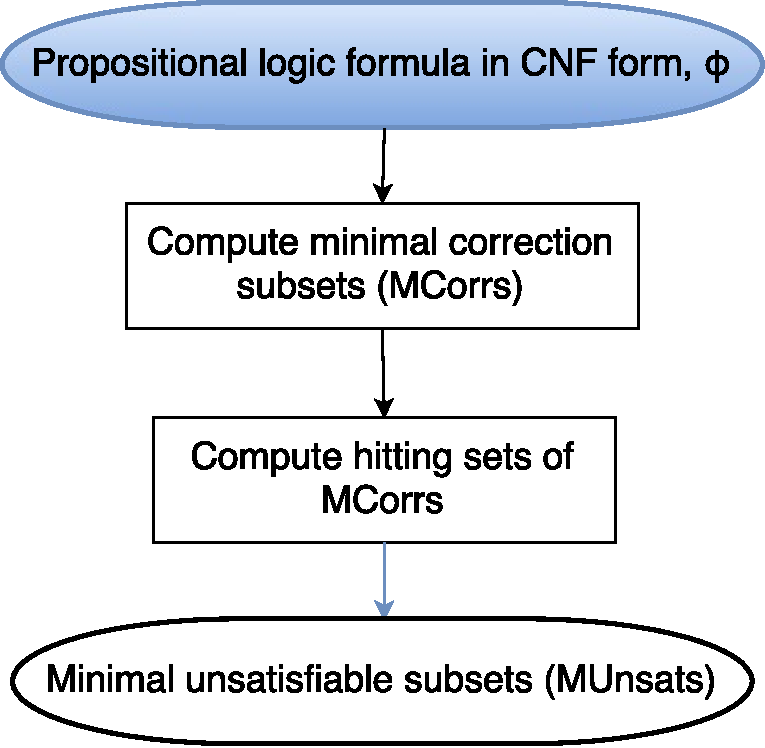
\includegraphics[scale=0.45]{FlowChartAll.pdf}
	\end{center}
\end{frame}

\begin{frame}{Propositional Logic Formula}
\begin{table}[]
	\centering
	\begin{tabular}{clcrcc}
		&\multicolumn{3}{c}{\visible<4->{$\overbrace{\visible<0>{aaaaaaaaaa}}\limits^{\only<4>{\color{blue}}clause}$}}  \\
		$\visible<5->{\varphi:=}$&$\visible<5->{(}\visible<1->{\only<1,3>{\color{blue}}\undernwarrow{x{\color{white}x}}}$     &   \visible<4->{$\vee$}   & $\visible<2->{\only<2,3>{\color{blue}}\undernearrow{\neg x}}\visible<5->{)}$     & \visible<5->{$\wedge$} & \visible<5->{$(x \vee \neg y)$}
		\only<1-2>{ \\ &\multicolumn{3}{c}{variable}}
		\only<3,4->{ \\ &\multicolumn{3}{c}{literals}}
		\only<1-5>{ \\ &\multicolumn{5}{l}{\visible<5>{$\underbrace{\visible<0>{aaaaaaaaaaaaaaaaaaaaaaaaaa}}\limits_{\text{\color{blue}conjunctive normal form}}$}}}
	\end{tabular}
\end{table}

\end{frame}

\begin{frame}{Problem Statement}
	\visible<1->{$\varphi:= (x
	\vee
	\neg x
	)\wedge(\neg 
	x \vee 
	y)$\\
	
	$\visible<0>{\varphi}:= (T
	\vee
	F
	)\wedge(
	F
	\vee 
	T)$\\
	$\visible<0>{\varphi}:= T\longrightarrow \text{ } ${\color{blue} SAT} \newline\newline}
	\visible<2->{
	$\varphi:={\only<3,4,5>{\color{green}}(x)}\wedge{{\only<3,5>{\color{green}}(\neg x)}}\wedge{{\only<4>{\color{green}}(\neg x\vee y)}}\wedge{{\only<3,4>{\color{green}}(\neg x \vee \neg y)}}$ \newline
	$\visible<0>{\varphi}:={({\color{red}T})}\wedge{({\color{red}F})}\wedge{({\color{red}F}\vee {\color{red}T})}\wedge{({\color{red}F} \vee {\color{red}F})}$ \newline
	$\visible<0>{\varphi}:= {\color{red}F}\longrightarrow \text{ }${\color{red} UNSAT}\newline
	\begin{table}[]
		\centering
		\begin{tabular}{lll}
			\visible<3-> {unsatisfiable subset & = & \{{\only<3>{\color{green}}$\hspace{1mm} \{(x),(\neg x),(\neg x \vee \neg y)\}$} \\}
			\visible<4-> {&   &,{\only<4>{\color{green}}$\{(x),(\neg x\vee y),(\neg x \vee \neg y)\}$}   \\}
			\visible<5-> {&   &  ,{\only<5>{\color{green}}$\{(x),(\neg x)\} \hspace{1mm}$}\}}
		\end{tabular}
	\end{table}
}
\end{frame}


\begin{frame}{Minimal Unsatisfiable Subsets and Minimal Correction Subsets}
	\begin{enumerate}[]
		\item <1-> \textbf{Minimal Unsatisfiable Subset (MUnsat):} 
		\begin{table}[]
			\centering
			\begin{tabular}{|c|c|c|c|c|c|}
				\hline
				($x$) & ($\neg x$) & ($\neg x \vee y$) & ($\neg x \vee \neg y$) & MUnsat & MinimumUnsat\\ \hline
				{\color{red}\lightning}   & {\color{red}\lightning}        &                &      & {\color{blue}\lightning}&{\color{cyan}\lightning} \\ \hline
				{\color{red}\lightning}   &   {\color{red}\lightning}      &           &          {\color{red}\lightning}   & & \\ \hline
				{\color{red}\lightning}   &         &        {\color{red}\lightning}        & {\color{red}\lightning} & {\color{blue}\lightning}  &\\  \hline
			\end{tabular}
		\end{table}
		\vspace*{\fill}
		\vspace*{\fill}
		\vspace*{\fill}
		\item <2-> \textbf{Minimal Correction Subset (MCorr):}
		\begin{table}[]
			\centering
			\begin{tabular}{|c|c|c|c|}
				\hline
				($x$) & ($\neg x$) & ($\neg x \vee y$) & ($\neg x \vee \neg y$) \\ \hline
				{\color{green}$\checkmark$}   &            &                &                     \\ \hline
				&    {\color{green}$\checkmark$}     &        {\color{green}$\checkmark$}        &              \\ \hline
				&    {\color{green}$\checkmark$}     &               &        {\color{green}$\checkmark$}      \\ \hline
			\end{tabular}
		\end{table}
	\end{enumerate}
	\vspace*{\fill}
	\vspace*{\fill}
	\vspace*{\fill}
	\vspace*{\fill}
	\vspace*{\fill}
	$$\varphi=\underbrace{(x)}\limits_{C_{1}}\wedge\underbrace{(\neg x)}\limits_{C_2}\wedge\underbrace{(\neg x\vee y)}\limits_{C_{3}}\wedge\underbrace{(\neg x \vee \neg y)}\limits_{C_{4}}$$
\end{frame}

\begin{frame}{Duality of Minimal Unsatisfiable and Correction Subset}
	\begin{itemize}
		\item \textbf{Hitting Sets:}
		\begin{enumerate}[]
			\item <1-> Variable Set: \hspace{5mm} D = $\{w, x, y, z\}$
			\item <1-> Collection Set: \hspace{2mm} $\Omega$ = $\{\{{\only<2>{\color{red}}{\only<6>{\color{red}}{\only<7>{\color{cyan}}w}}},
			{\only<2>{\color{black}}{\only<3>{\color{green}}{\only<4>{\color{cyan}}{\only<8>{\color{green}}x}}}}\},
			\{{\only<2>{\color{black}}{\only<3>{\color{green}}{\only<4>{\color{cyan}}{\only<8>{\color{green}}x}}}},
			{\only<3>{\color{green}}{\only<6>{\color{red}}y}},{\only<2>{\color{red}}{\only<7>{\color{cyan}}z}}\}\}$
			
			\item <1-> Hitting Set: \hspace{7mm} $H = \{\{{\only<2>{\color{red}}w},{\only<2>{\color{red}}z}\}, \{{\only<3>{\color{green}}x},{\only<3>{\color{green}}y}\}, \{{\only<4>{\color{cyan}}x}\}, $ \ldots $\}$
			
			
			\item <5-> Minimal Hitting Set: $MinH = \{\{{\only<6>{\color{red}}w},{\only<6>{\color{red}}y}\}, \{{\only<7>{\color{cyan}}w},{\only<7>{\color{cyan}}z}\}, {\only<8>{\color{green}}x}\}     $                          
		\end{enumerate}
		\item \visible<9->{ Minimal hitting sets of the set of MCorr:
		\begin{figure}[]
	\begin{center}
		\begin{tikzpicture}[scale=1.5, 
		state/.style={draw, rounded corners, fill=none,
			text centered, text=black}]
		\node[] (u0) at (1, 2) {MCorr};
		\node[state] (u1) at (2, 2) {\only<10>{\color{red}}{\only<9>{\color{blue}}$C_{1}$}};
		\node[state] (u2) at (4, 2) {${{\only<9>{\color{blue}}C_{2}}}, {\only<10>{\color{red}}C_{3}}$};
		\node[state] (u3) at (6, 2) {${\only<9>{\color{blue}}C_{2}}, {\only<10>{\color{red}}C_{4}}$};
		\node[state] (u4) at (3, 1) {{\only<9>{\color{blue}}$C_{1}, C_{2}$}};
		\node[state] (u5) at (5, 1) {${\only<10>{\color{red}}C_{1}}, {\only<10>{\color{red}}C_{3}}, {\only<10>{\color{red}}C_{4}}$};
		\node[] (u6) at (1, 1) {MUnsat};
		
		\path[<->] 	(u1)  edge   (u4);
		\path[<->] 	(u1)  edge   (u5);
		\path[<->] 	(u2)  edge   (u4);
		\path[<->] 	(u2)  edge   (u5);
		\path[<->] 	(u3)  edge   (u4);
		\path[<->] 	(u3)  edge   (u5);
		\end{tikzpicture}
	\end{center}
\end{figure}}
	\end{itemize}
	\only<9->{$$\varphi=\underbrace{(x)}\limits_{C_{1}}\wedge\underbrace{(\neg x)}\limits_{C_2}\wedge\underbrace{(\neg x\vee y)}\limits_{C_{3}}\wedge\underbrace{(\neg x \vee \neg y)}\limits_{C_{4}}$$}
\end{frame}

\begin{frame}{FlowChart}
	\begin{center}
		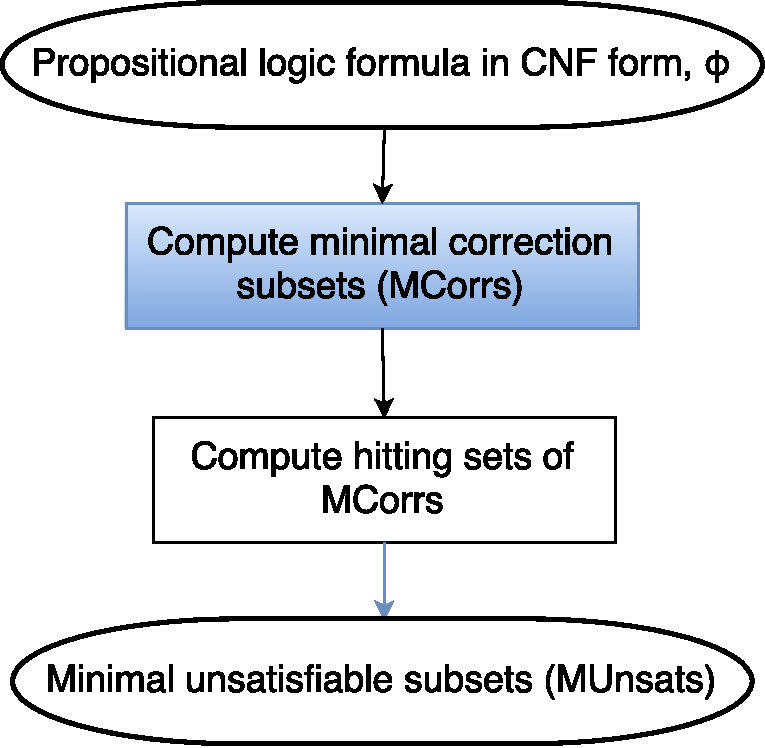
\includegraphics[scale=0.45]{FlowChartAll-1.pdf}
	\end{center}
\end{frame}

\begin{frame}{Algorithm: Computing all MCorrs}
	\begin{enumerate}
		\item <1-> Augment CNF with clause selector variables
		\begin{table}[]
			\centering
			\scalebox{.8}{
			\begin{tabular}{ccccccccc}
				$\varphi=$& $(x)$ & $\wedge$ & $(\neg x)$ & $\wedge$ & $(\neg x\vee y)$ & $\wedge$ & $(\neg x \vee \neg y)$&  \\
				$\varphi^{\prime}=$& $({\only{\color{red}}\neg w_{1}}\vee x)$ & $\wedge$ & $({\only{\color{red}}\neg w_{2}}\vee \neg x)$ & $\wedge$ & $({\only{\color{red}}\neg w_{3}}\vee \neg x\vee y)$ & $\wedge$ & $({\only{\color{red}}\neg w_{4}} \vee \neg x \vee \neg y)$ & 
			\end{tabular}}
		\end{table}
		\item <2-> All MCorrs are found incrementally
				$$\varphi^{\prime}=(\neg {\only{\color{green}}\mathbf{false}} \vee x)\text{ }\wedge\text{ }(\neg w_{2}\vee \neg x)\text{ }\wedge\text{ }(\neg w_{3}\vee \neg x\vee y)\text{ }\wedge\text{ }(\neg w_{4}\vee \neg x \vee \neg y)$$
		\item <3-> Add blocking clauses to block old solutions
		$$\varphi^{\prime}=\varphi^{\prime} \wedge {\only{\color{cyan}} w_{1}}$$
	\end{enumerate}
\end{frame}

\begin{frame}{Example: Computing all MCorrs}

	\begin{tabular}{lll}
		$\varphi$& $=$ & $({\only{\color{red}}\only<2->{\neg w_{1}\vee}} x)\wedge({\only{\color{red}}\only<2->{\neg w_{2}\vee}} \neg x)\wedge({\only{\color{red}}\only<2->{\neg w_{3}\vee}}\neg x\vee y)\wedge({\only{\color{red}}\only<2->{\neg w_{4}\vee}}\neg x \vee \neg y)$ \\
		&  & $\only<4->{\wedge{\only{\color{green}}(w_{1})}}\text{ } \only<6->{{\wedge\text{ }\only{\color{green}}(w_{2} \vee w_{3})}} \only<7->{\wedge{\only{\color{green}}(w_{2} \vee w_{4})}}$
	\end{tabular}

\visible<2->{
\begin{tabular}{|p{6cm}|}
	\hline
	\fontsize{9}{9}\selectfont
	\begin{enumerate}
		\item <2-> Add clause-selector variables.
		\item <3-> Add AtMost constraint.
		\item <4-> First solution : $w_{1}$ is $\mathbf{false}$. Add blocking clause and a MCorr.
		\item <5-> No further solutions, increment AtMost.
		\item <6-> Second solution : $w_{2}$ and $w_{3}$ are $\mathbf{false}$. Add blocking clause and another MCorrs.
		\item <7-> Third solution : $ w_{2} $ and $ w_{4} $ are $\mathbf{false}$. Add blocking clause and another MCorrs.
		\item <8-> No further solutions, even without AtMost constraint.
	\end{enumerate}\\
	\hline
\end{tabular}
\visible<4->{
\fbox{
	\begin{minipage}{8em}{MCorrs}
		\fontsize{7.6}{9}\selectfont
		\begin{enumerate}
			\item <4-> ${\only{\color{cyan}}\{(x)\}}$
			\item <6-> ${\only{\color{cyan}}\{(\neg x), (\neg x\vee y) \}}$
			\item <7-> ${\only{\color{cyan}}\{(\neg x), (\neg x\vee \neg y) \}}$
		\end{enumerate}
	\end{minipage}
} }}
\visible<3-7>{$$AtMost(\{w_{1},w_{2},w_{3},w_{4}\}, \only<3-4>{1} \only<5-7>{2} )$$}
\end{frame}
\begin{frame}{FlowChart}
	\begin{center}
		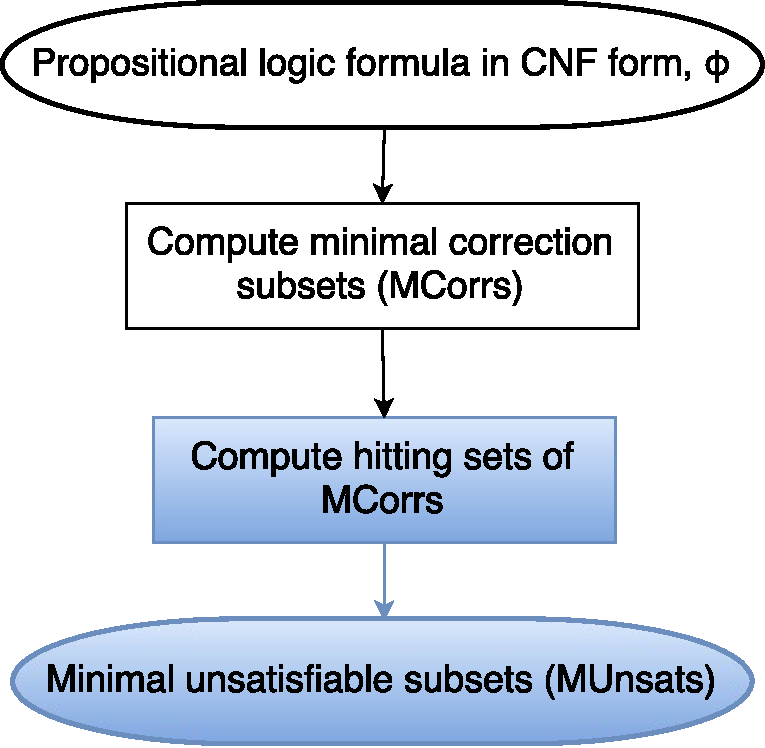
\includegraphics[scale=0.45]{FlowChartAll-2.pdf}
	\end{center}
\end{frame}
\begin{frame}{Example: Computing All Minimal Hitting Sets of MUnsats}
	\begin{center}

		\only<1>{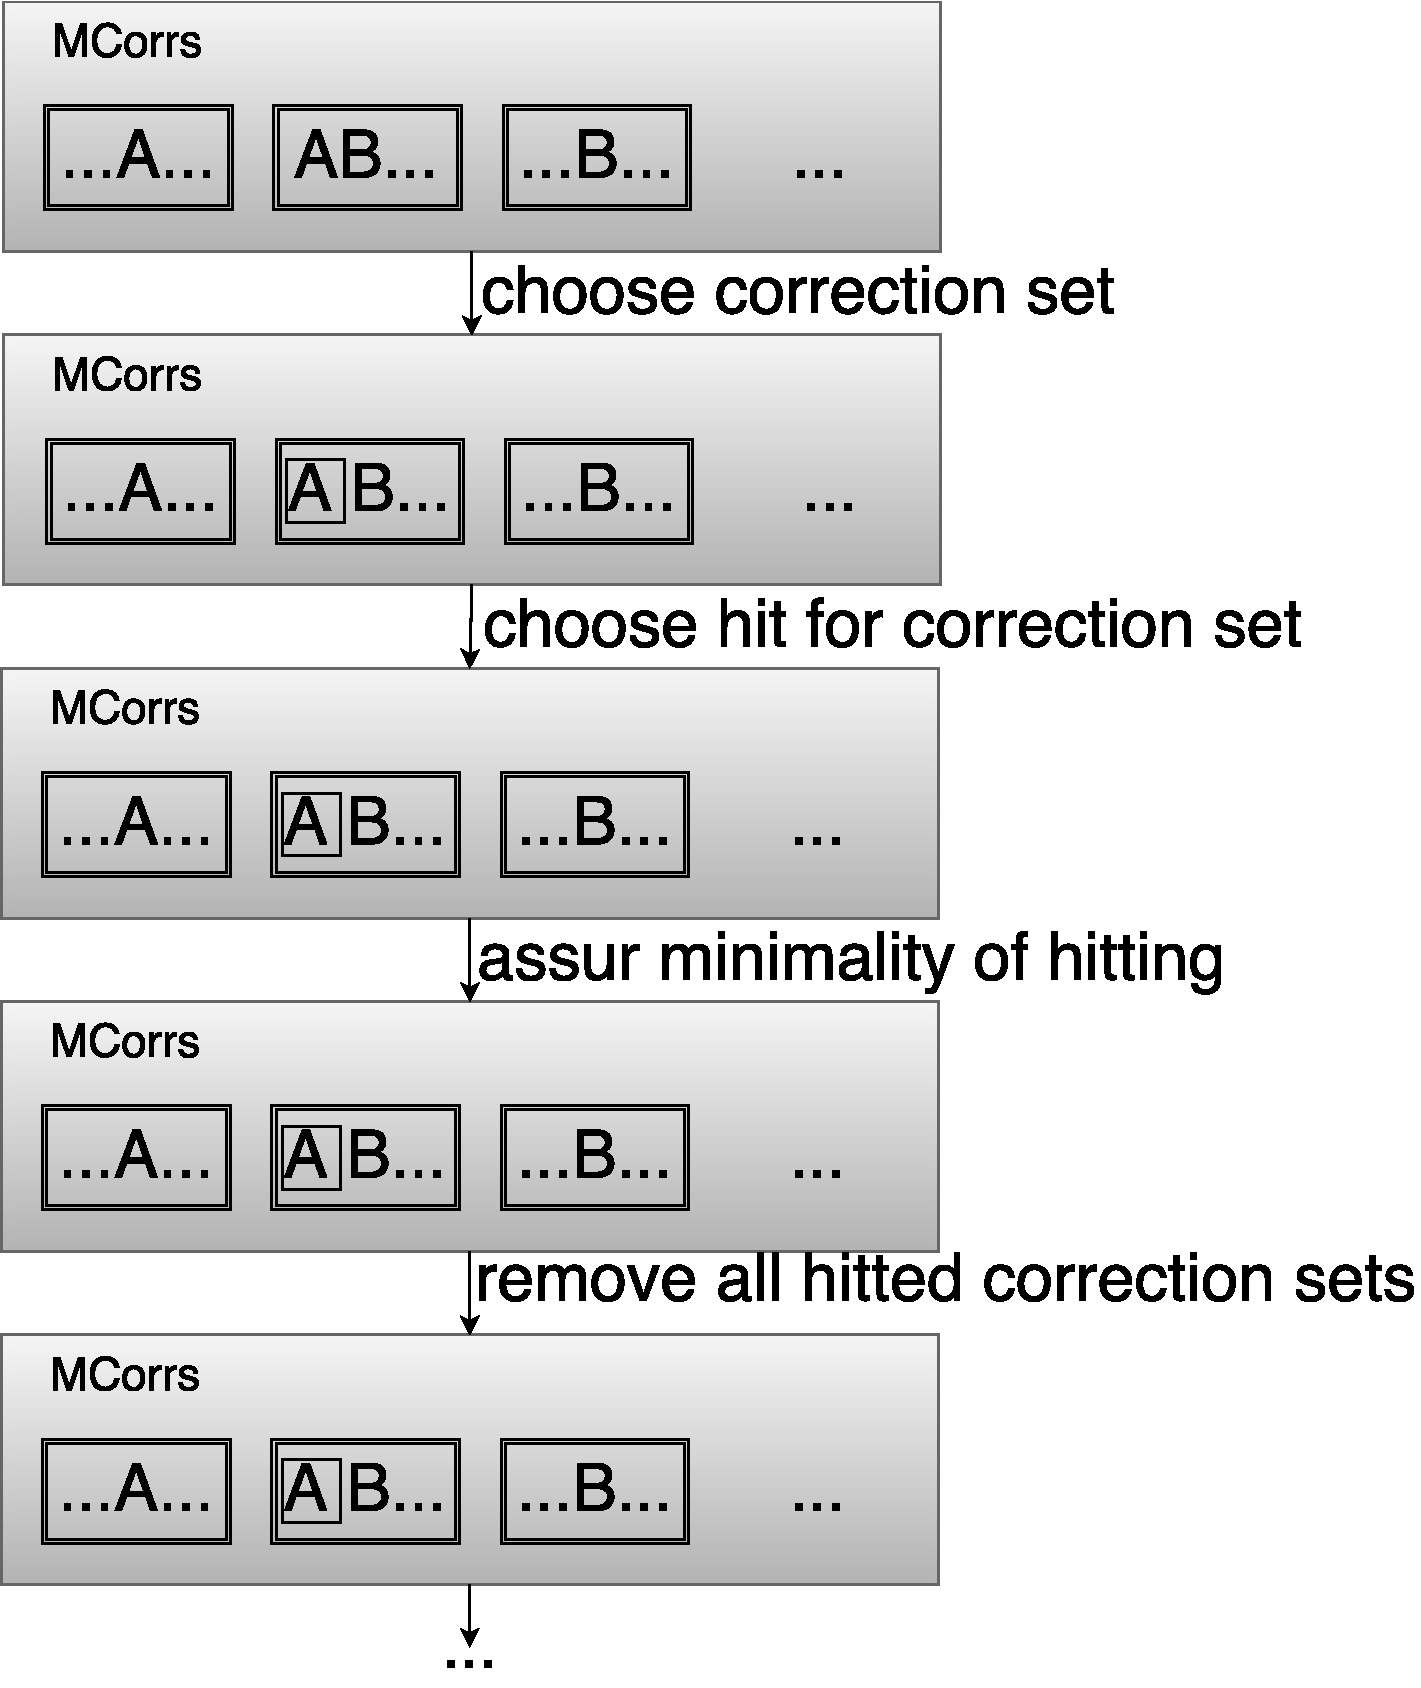
\includegraphics[scale=0.26]{HittingSets1.pdf}}
		\only<2>{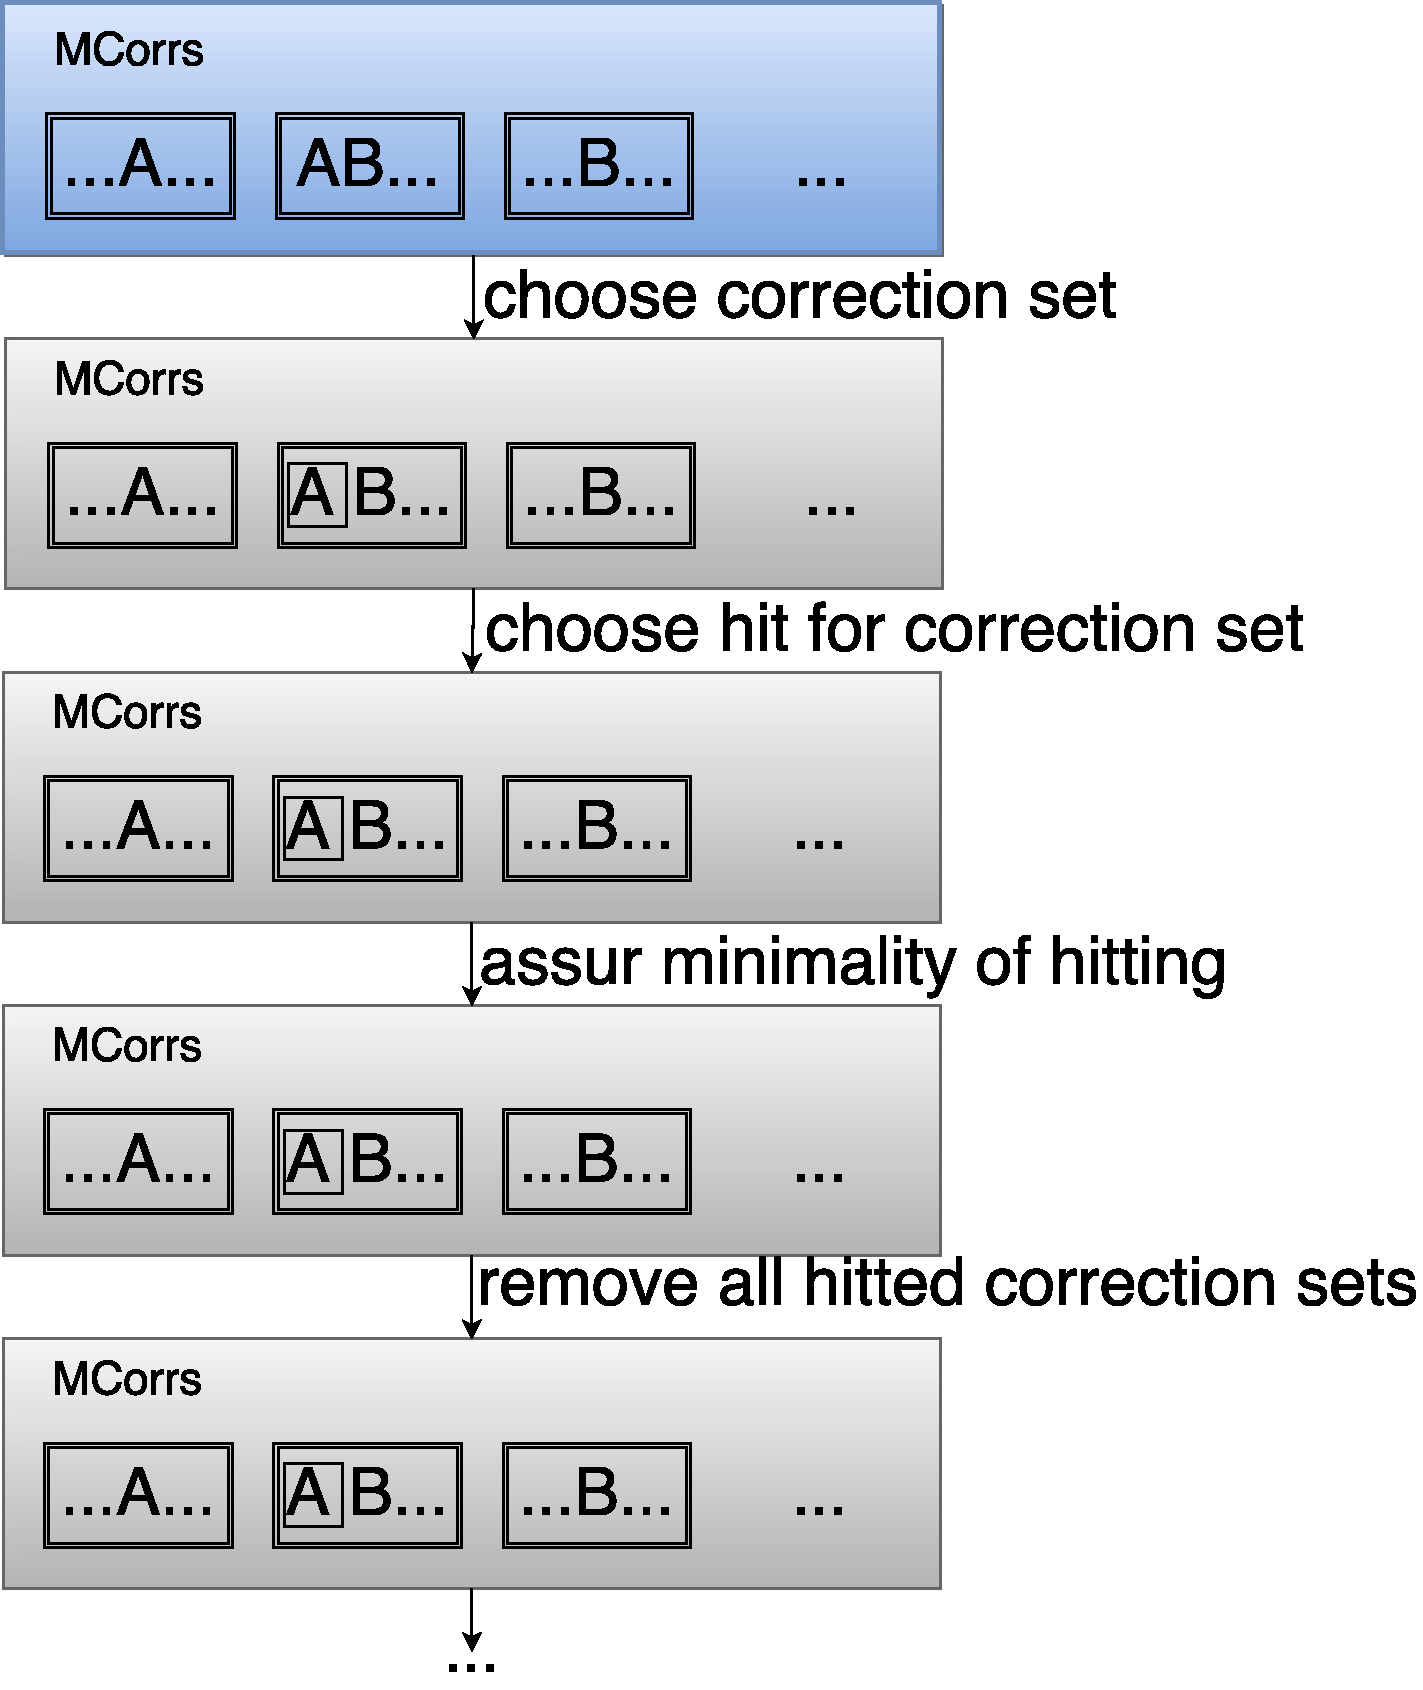
\includegraphics[scale=0.26]{HittingSets2.pdf}}
		\only<3>{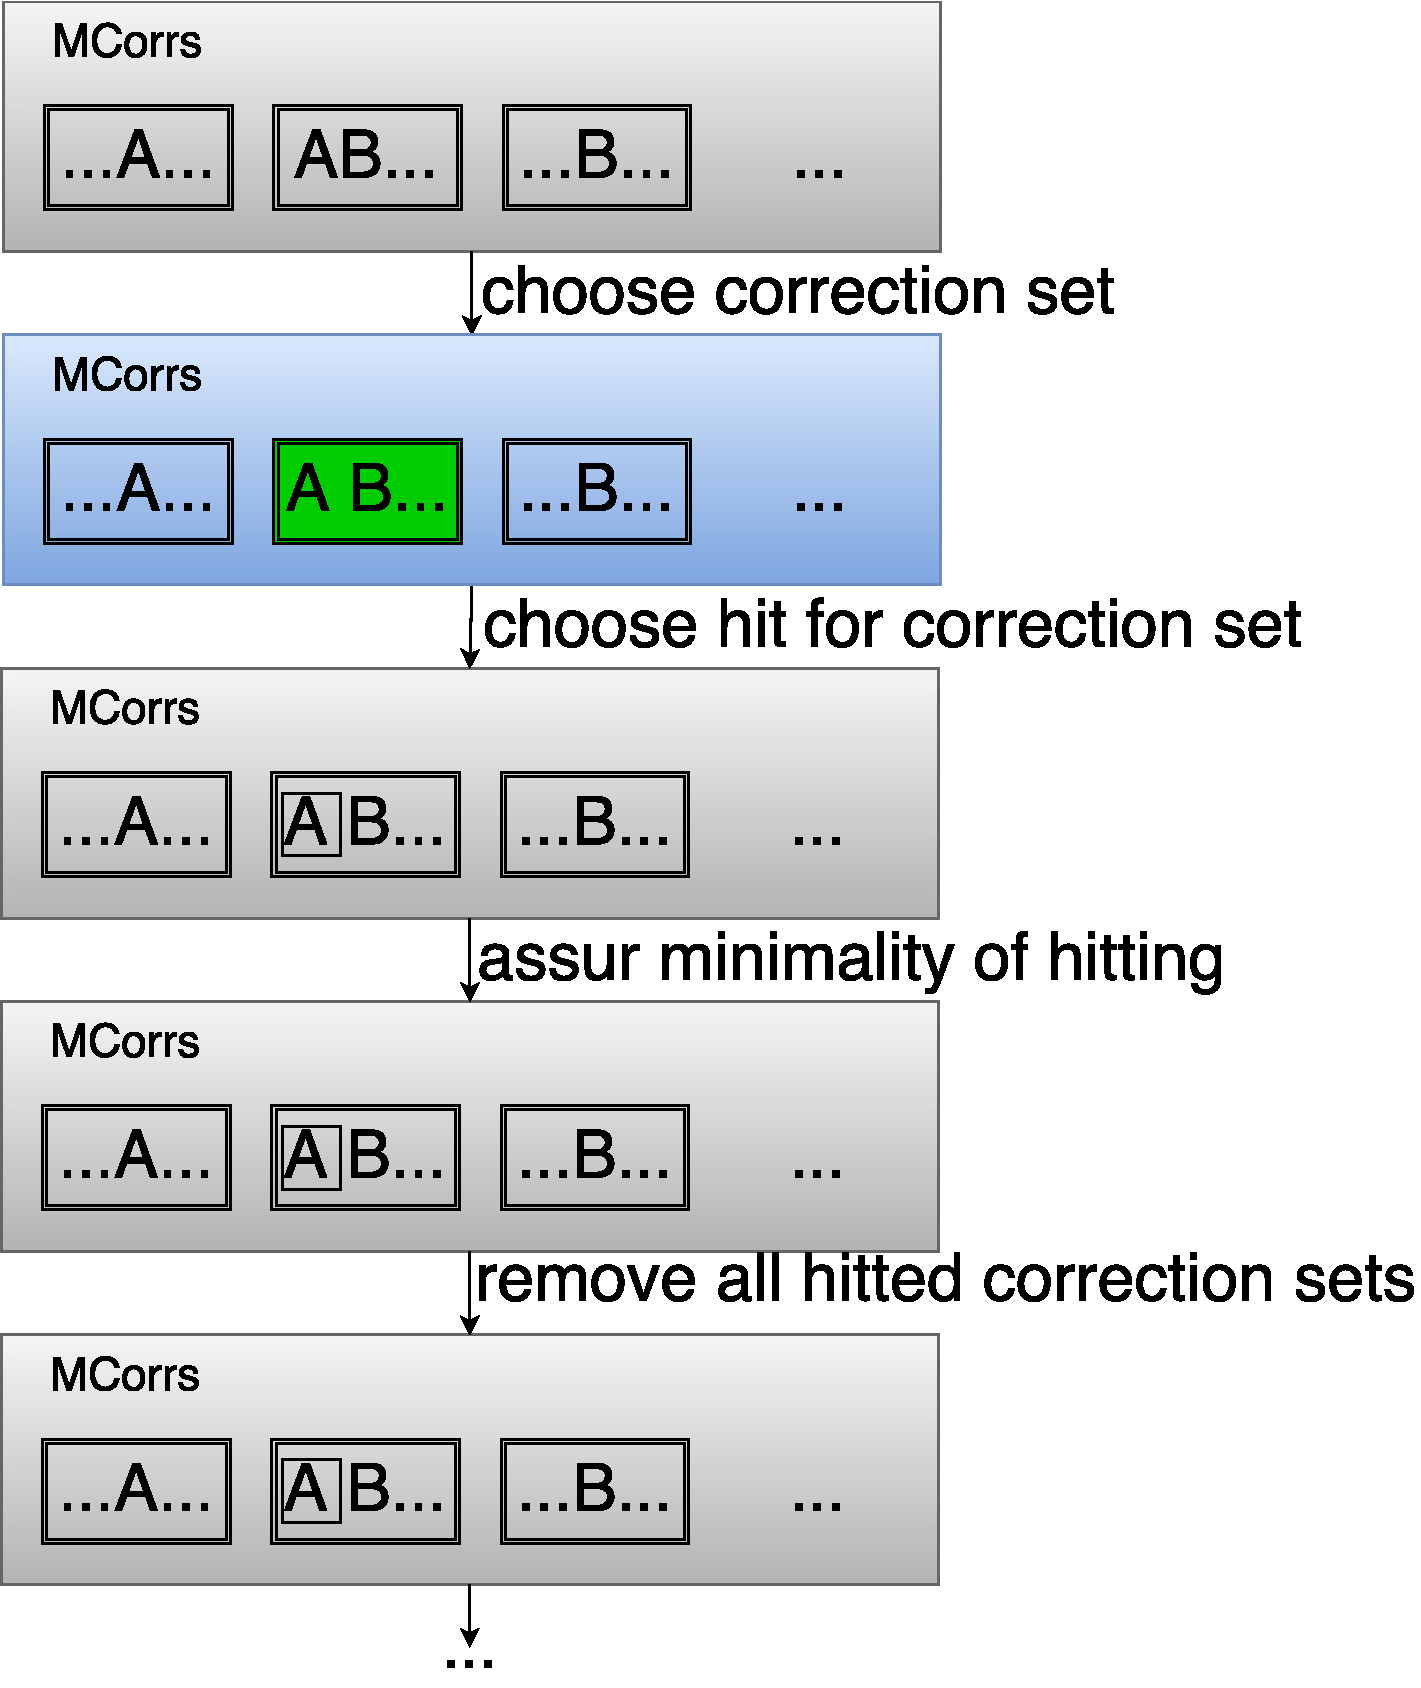
\includegraphics[scale=0.26]{HittingSets3.pdf}}
		\only<4>{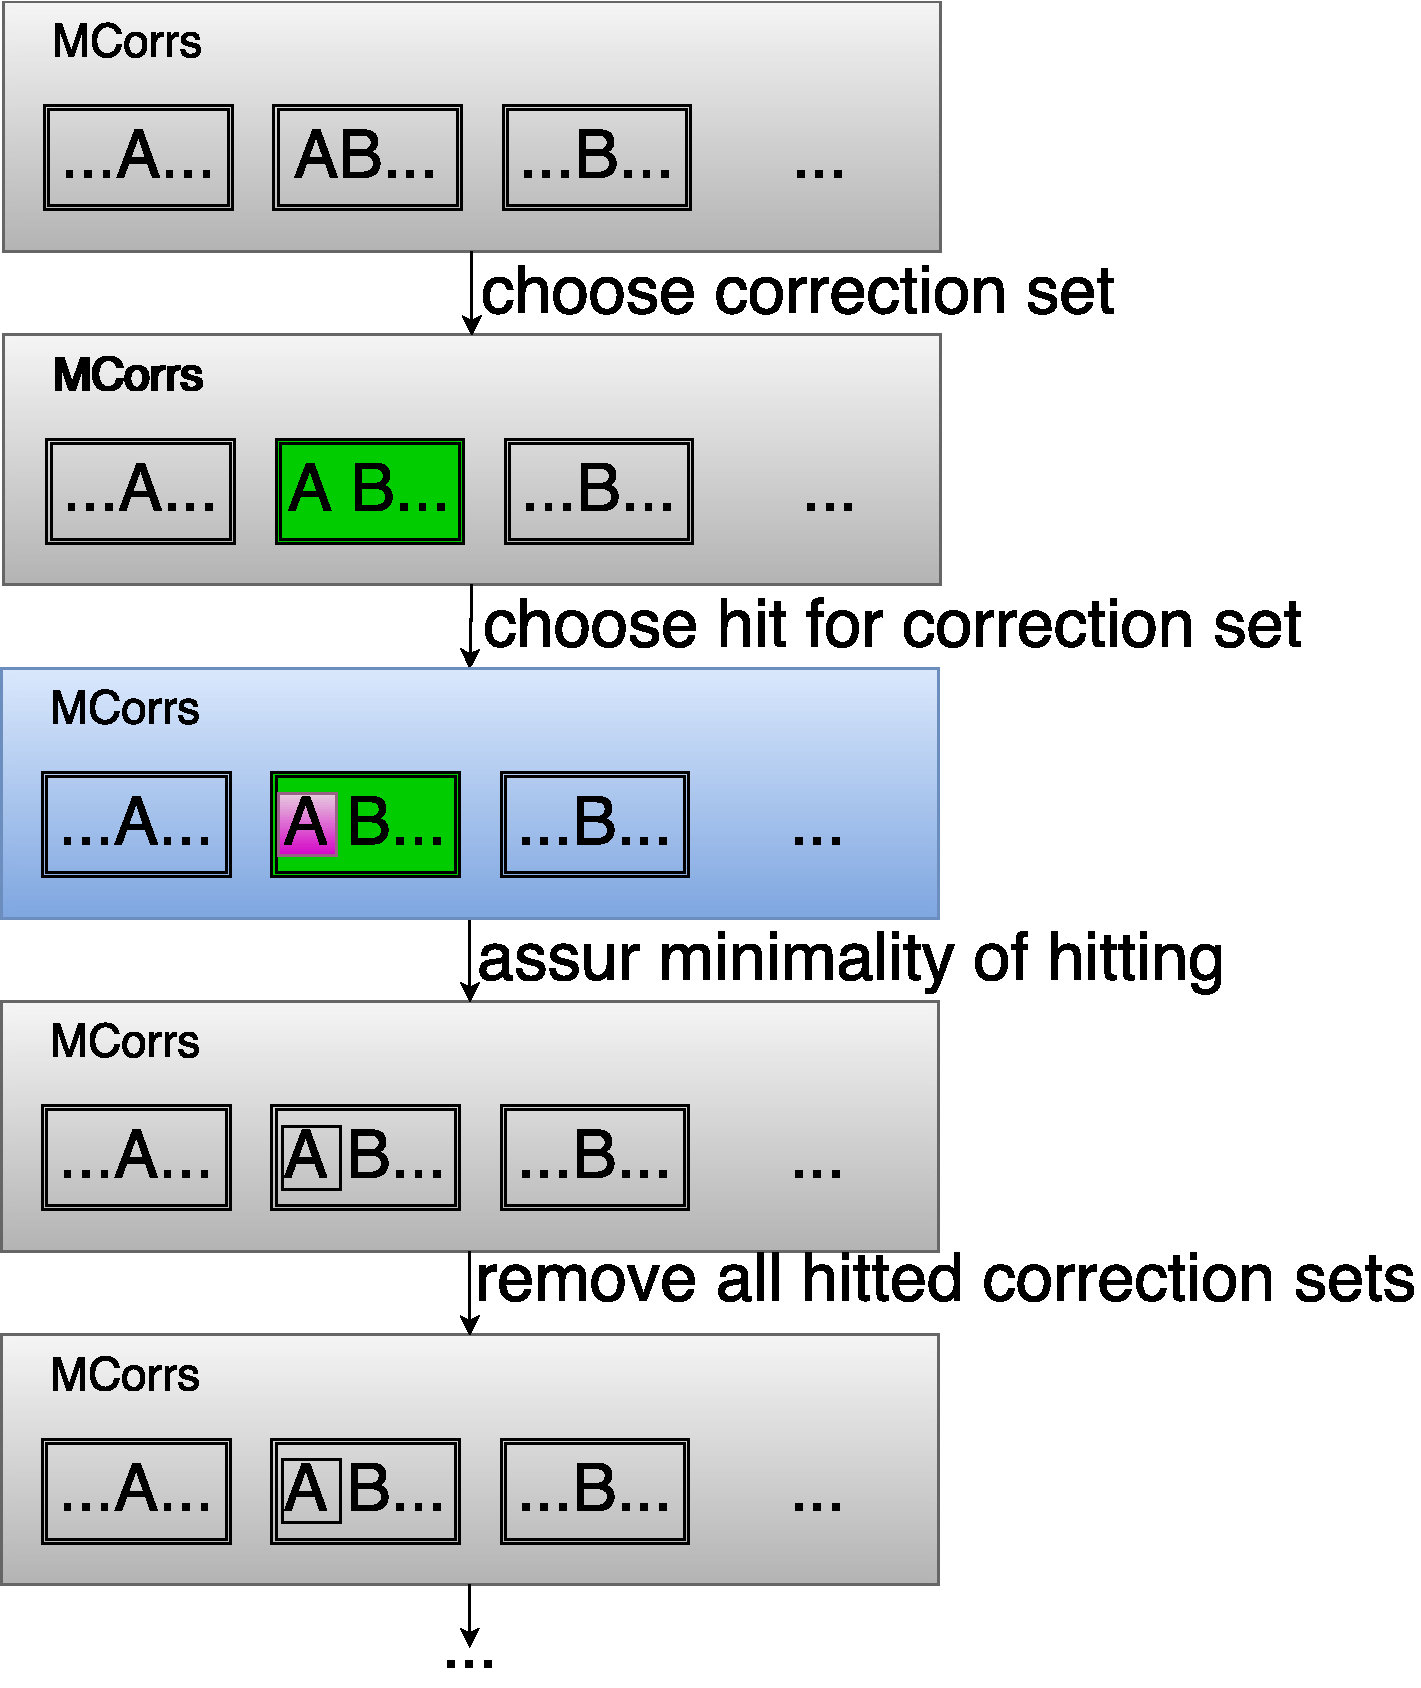
\includegraphics[scale=0.26]{HittingSets4.pdf}}
		\only<5>{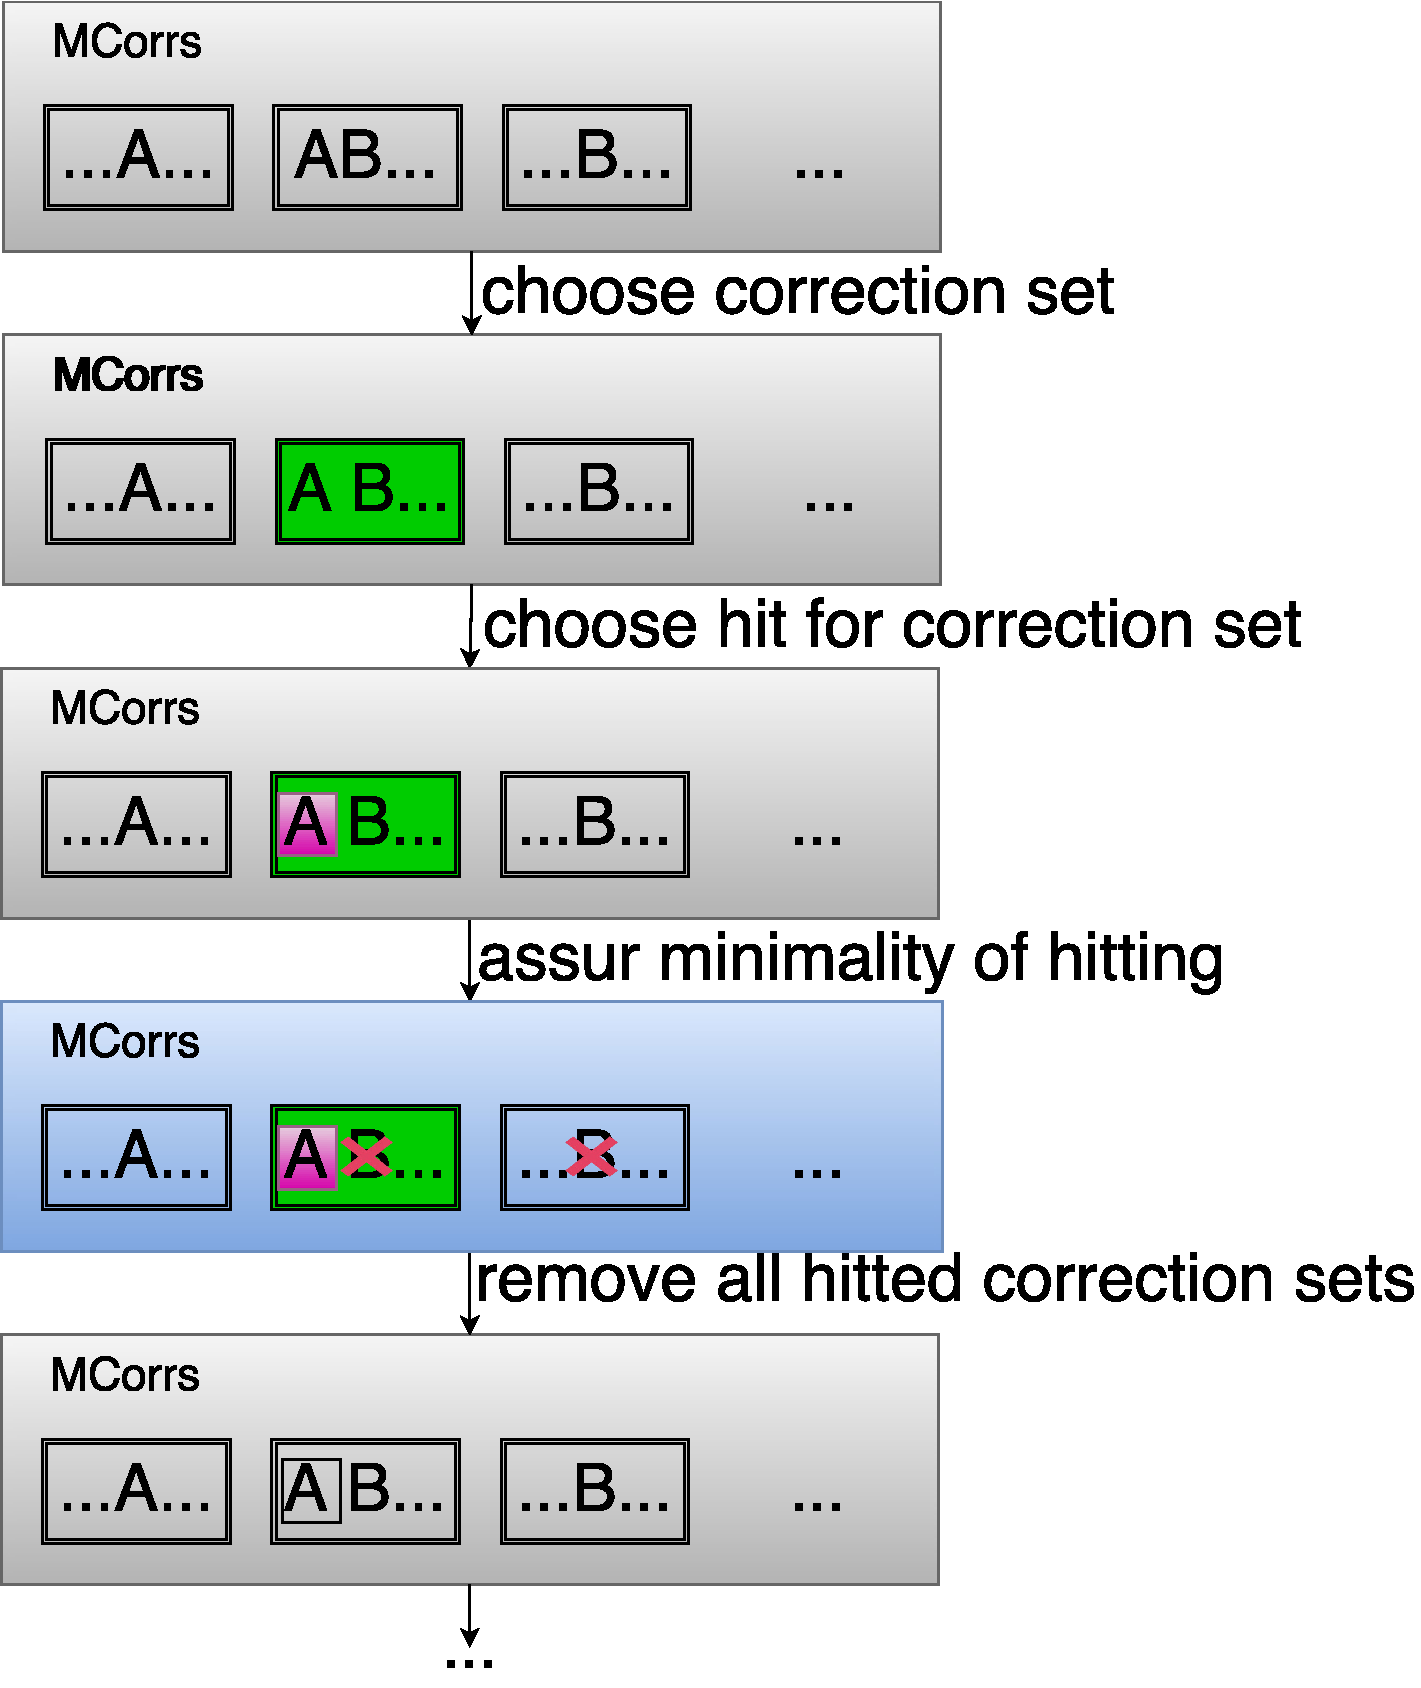
\includegraphics[scale=0.26]{HittingSets5.pdf}}
		\only<6>{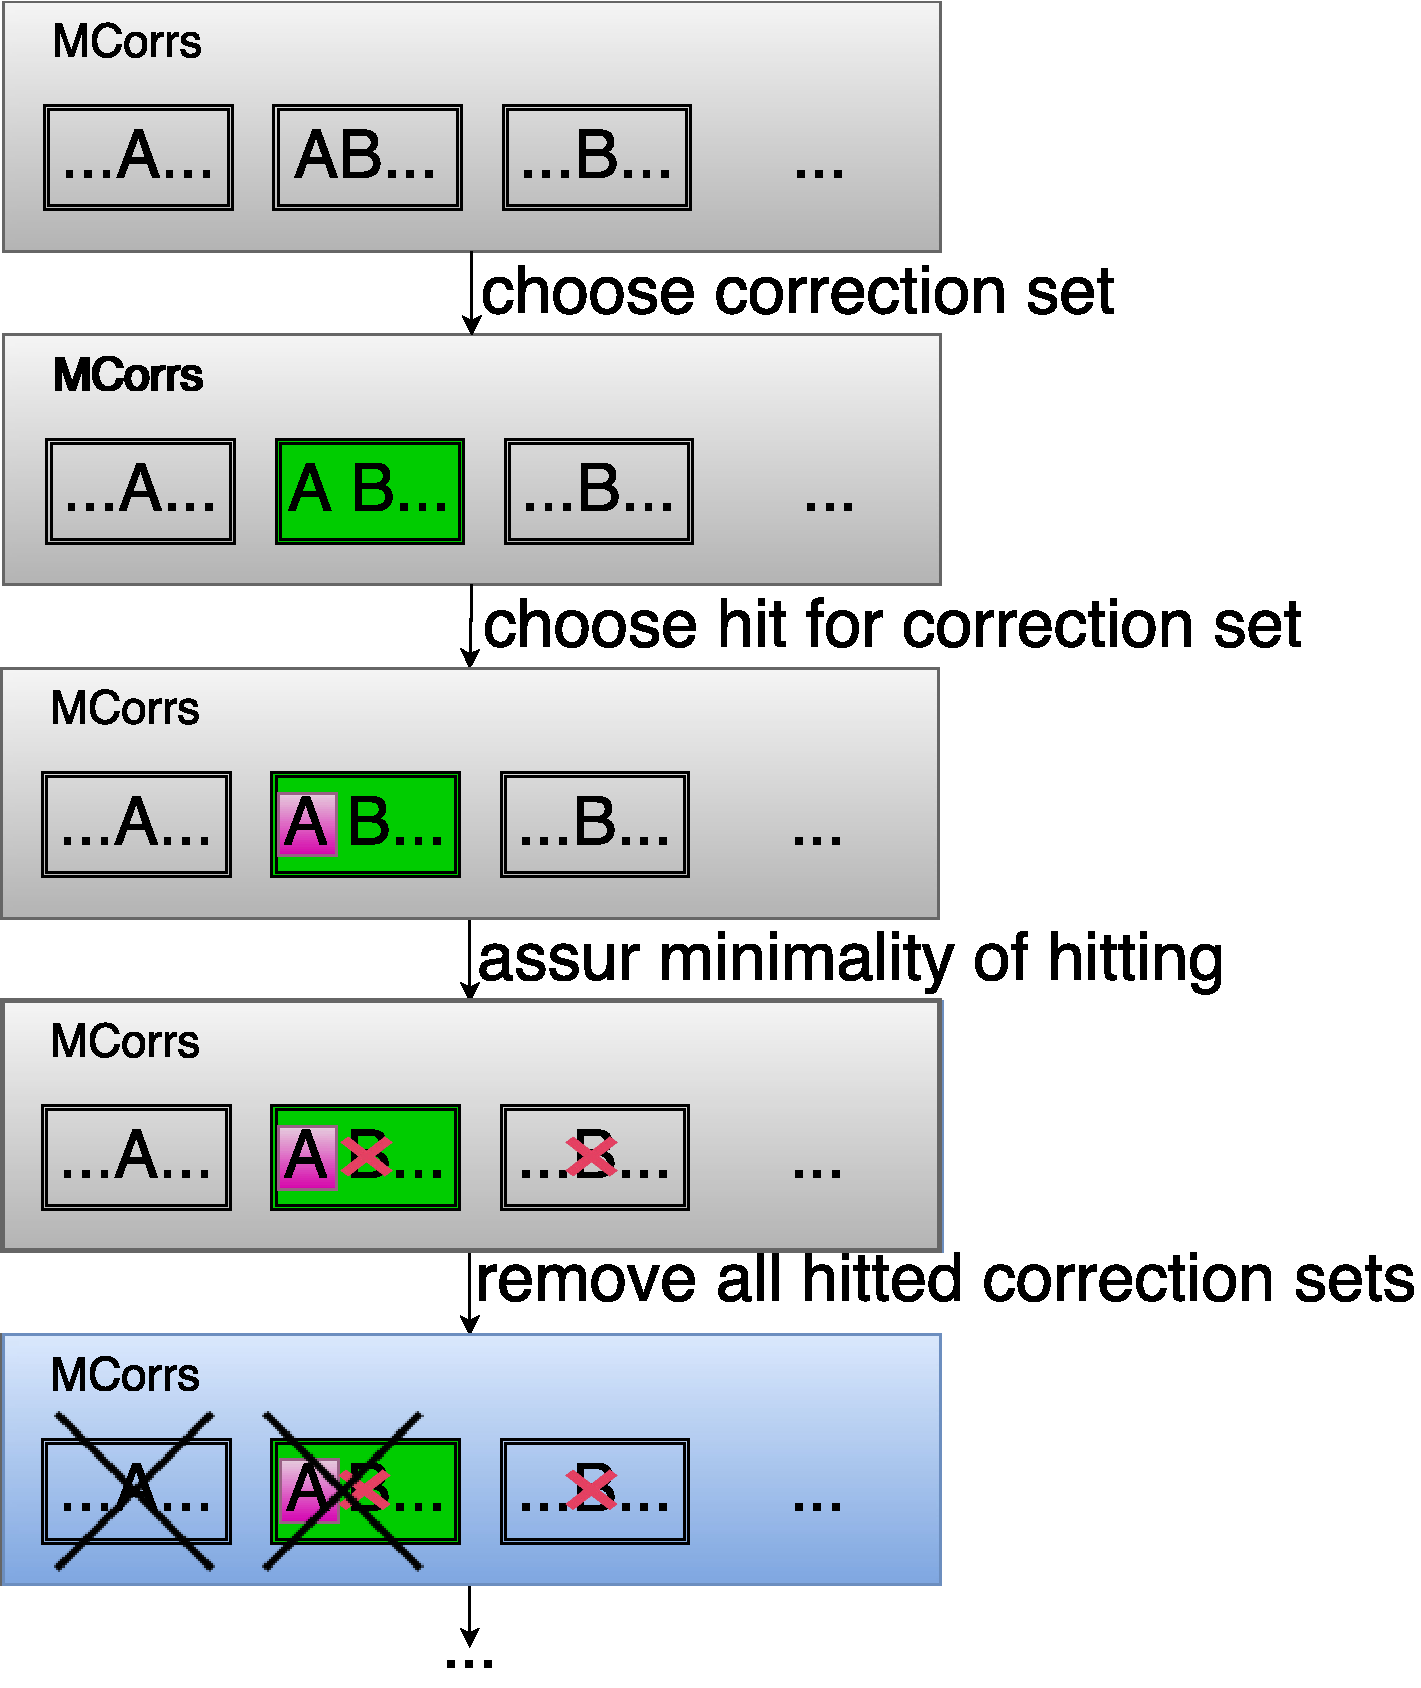
\includegraphics[scale=0.26]{HittingSets6.pdf}}
	\end{center}
\end{frame}
\begin{frame}{Example: Computing All Hitting Sets of MUnsats}
	\begin{center}
		\only<1>{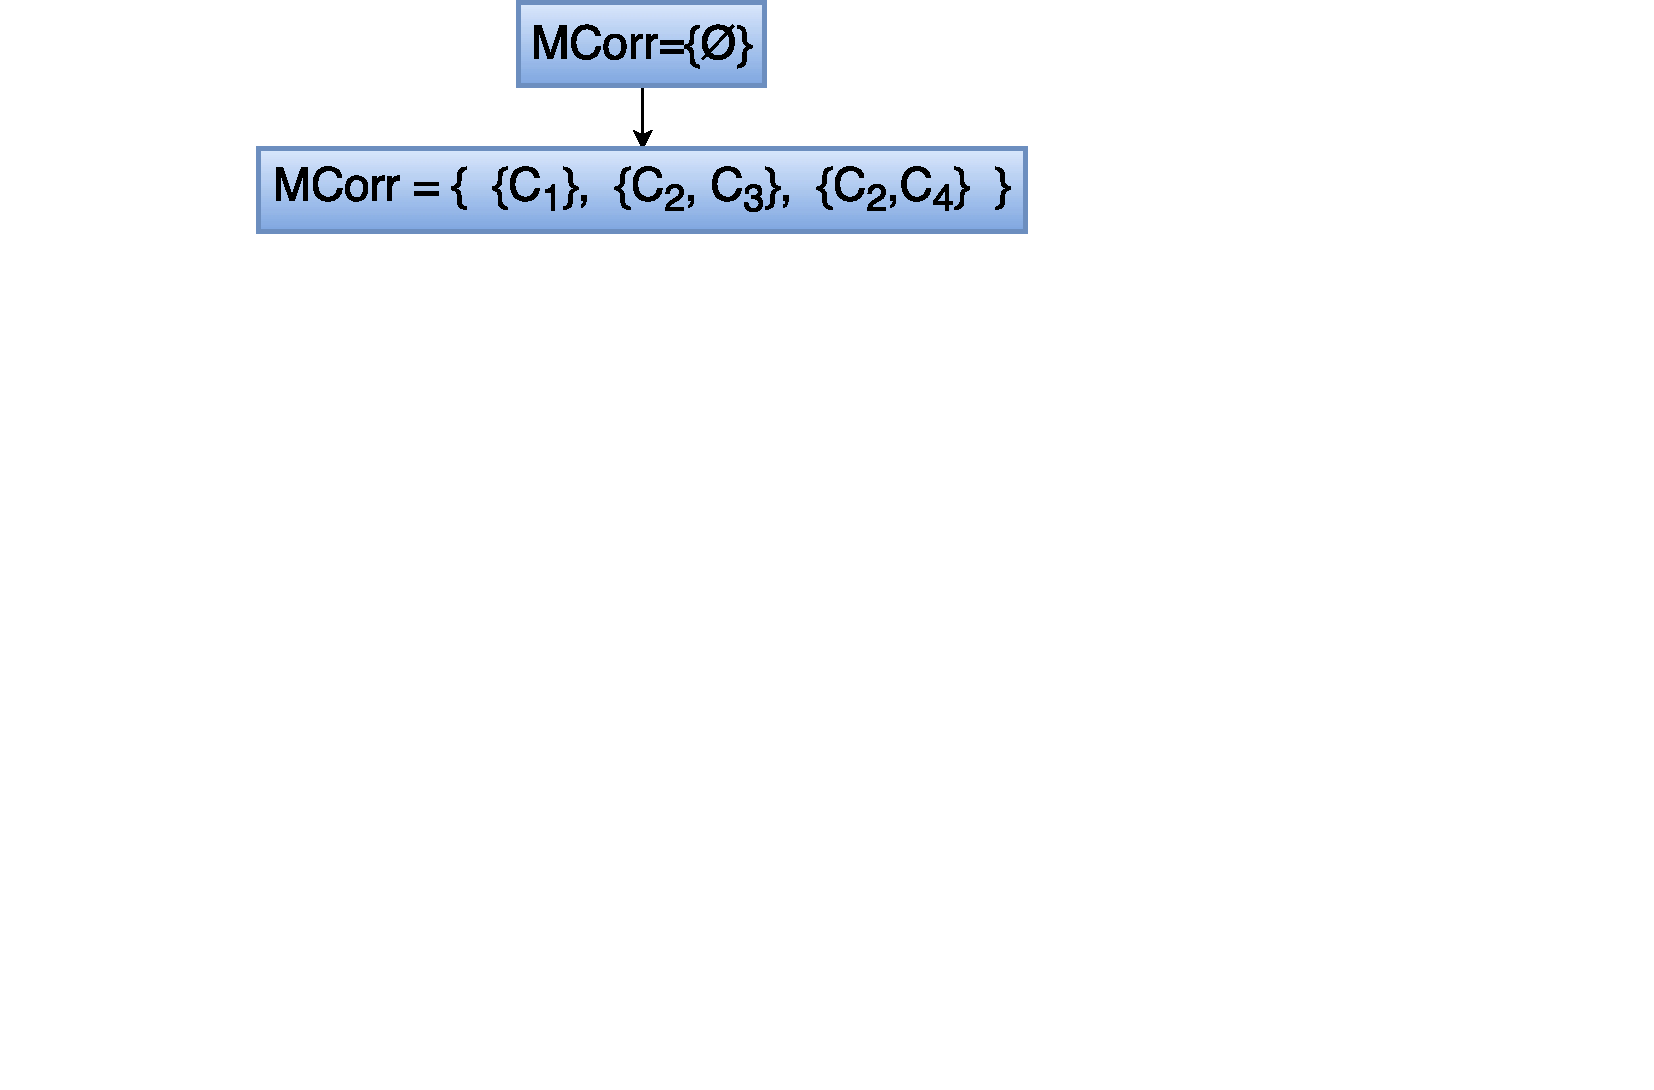
\includegraphics[scale=0.38]{HittingSetAlgo1.pdf}}
		\only<2>{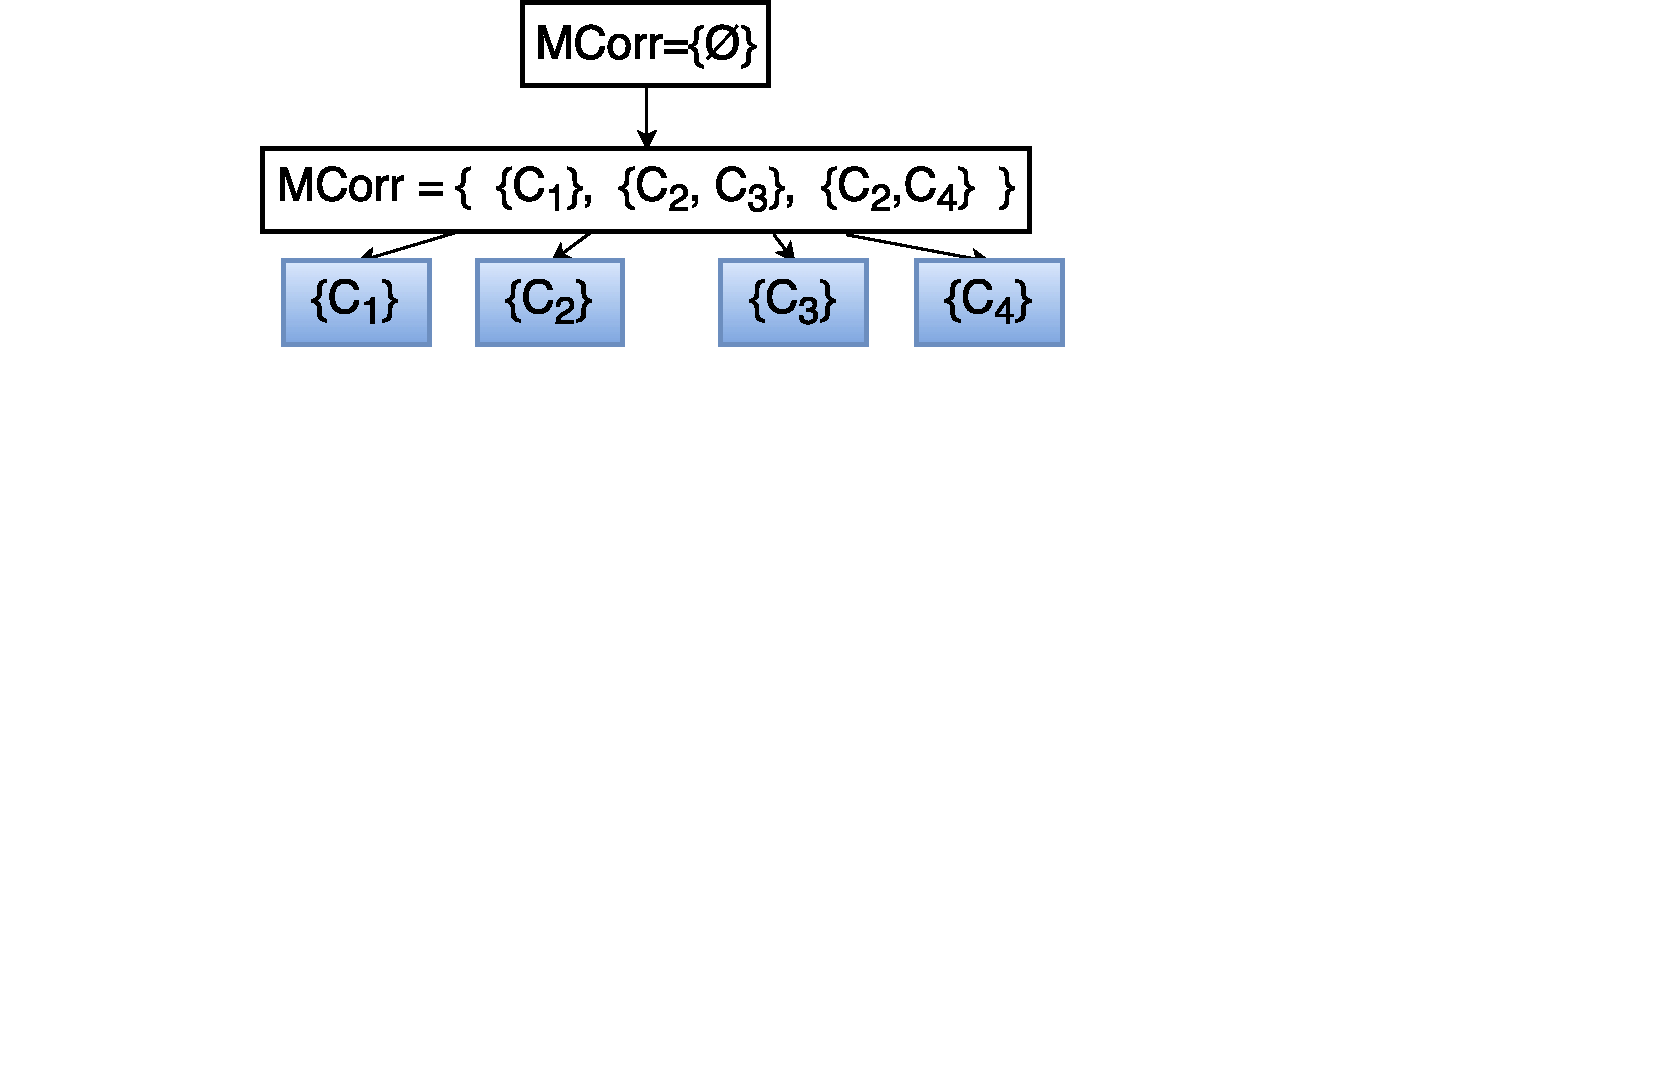
\includegraphics[scale=0.38]{HittingSetAlgo2.pdf}}
		\only<3>{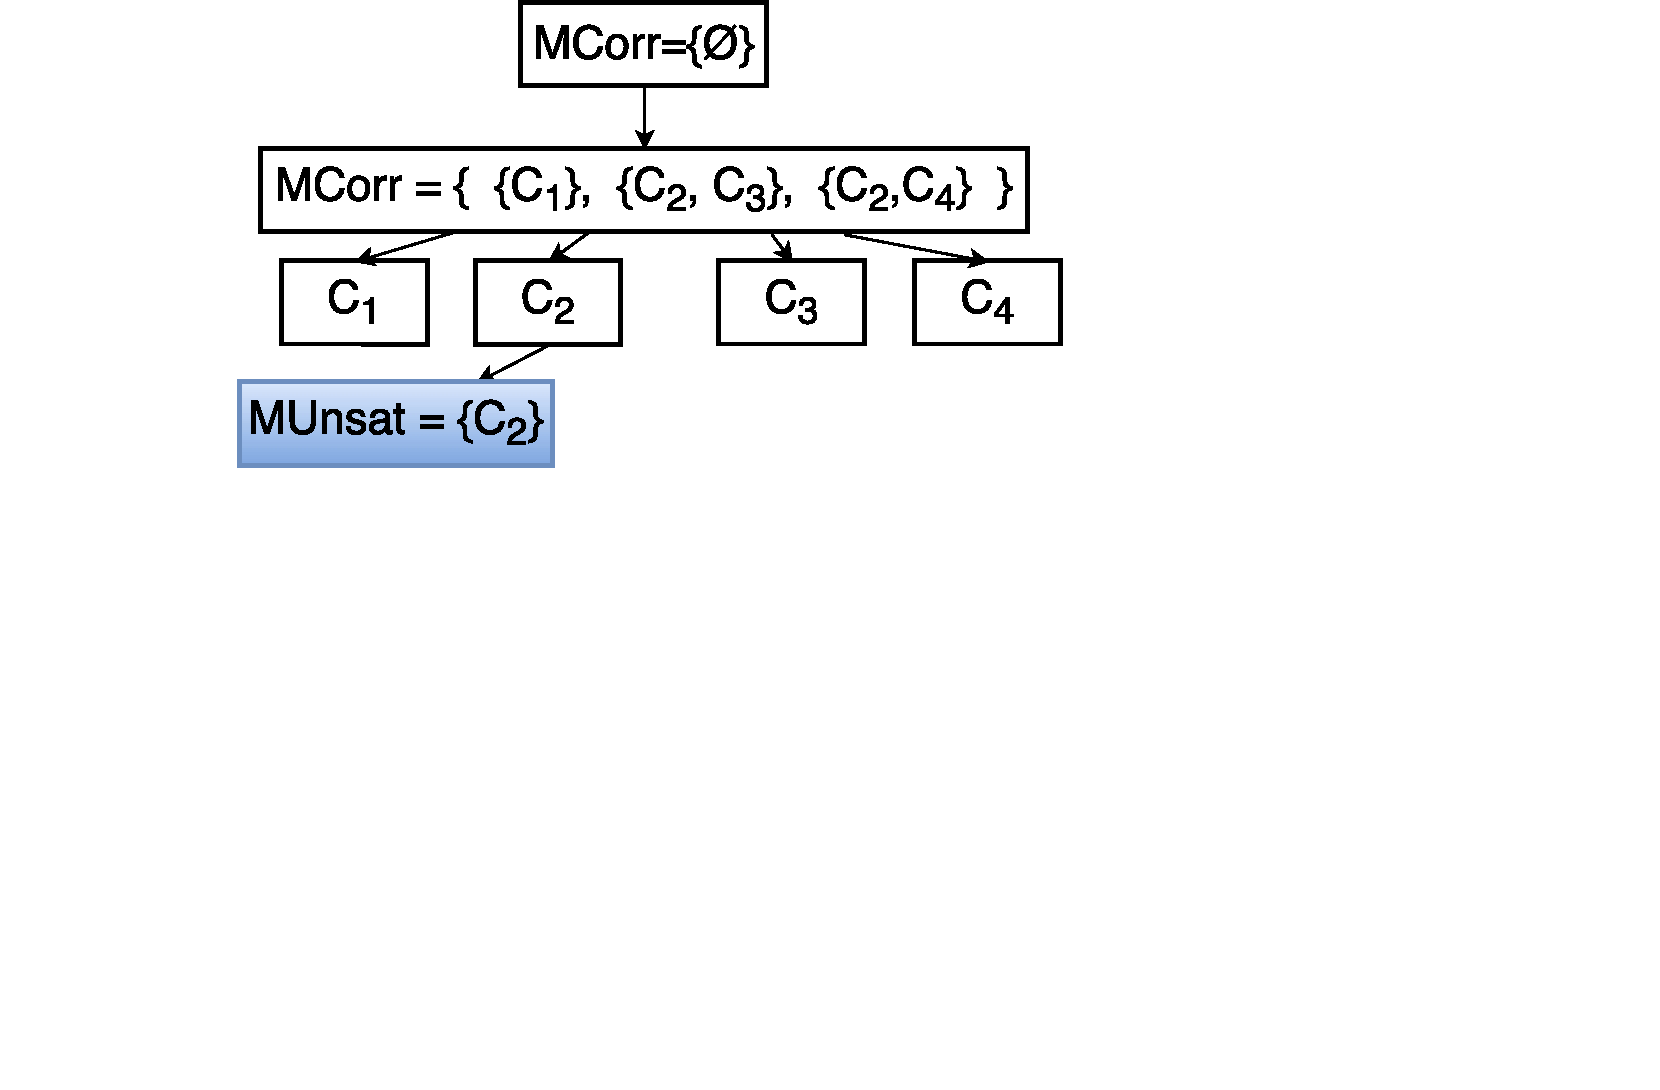
\includegraphics[scale=0.38]{HittingSetAlgo3.pdf}}
		\only<4>{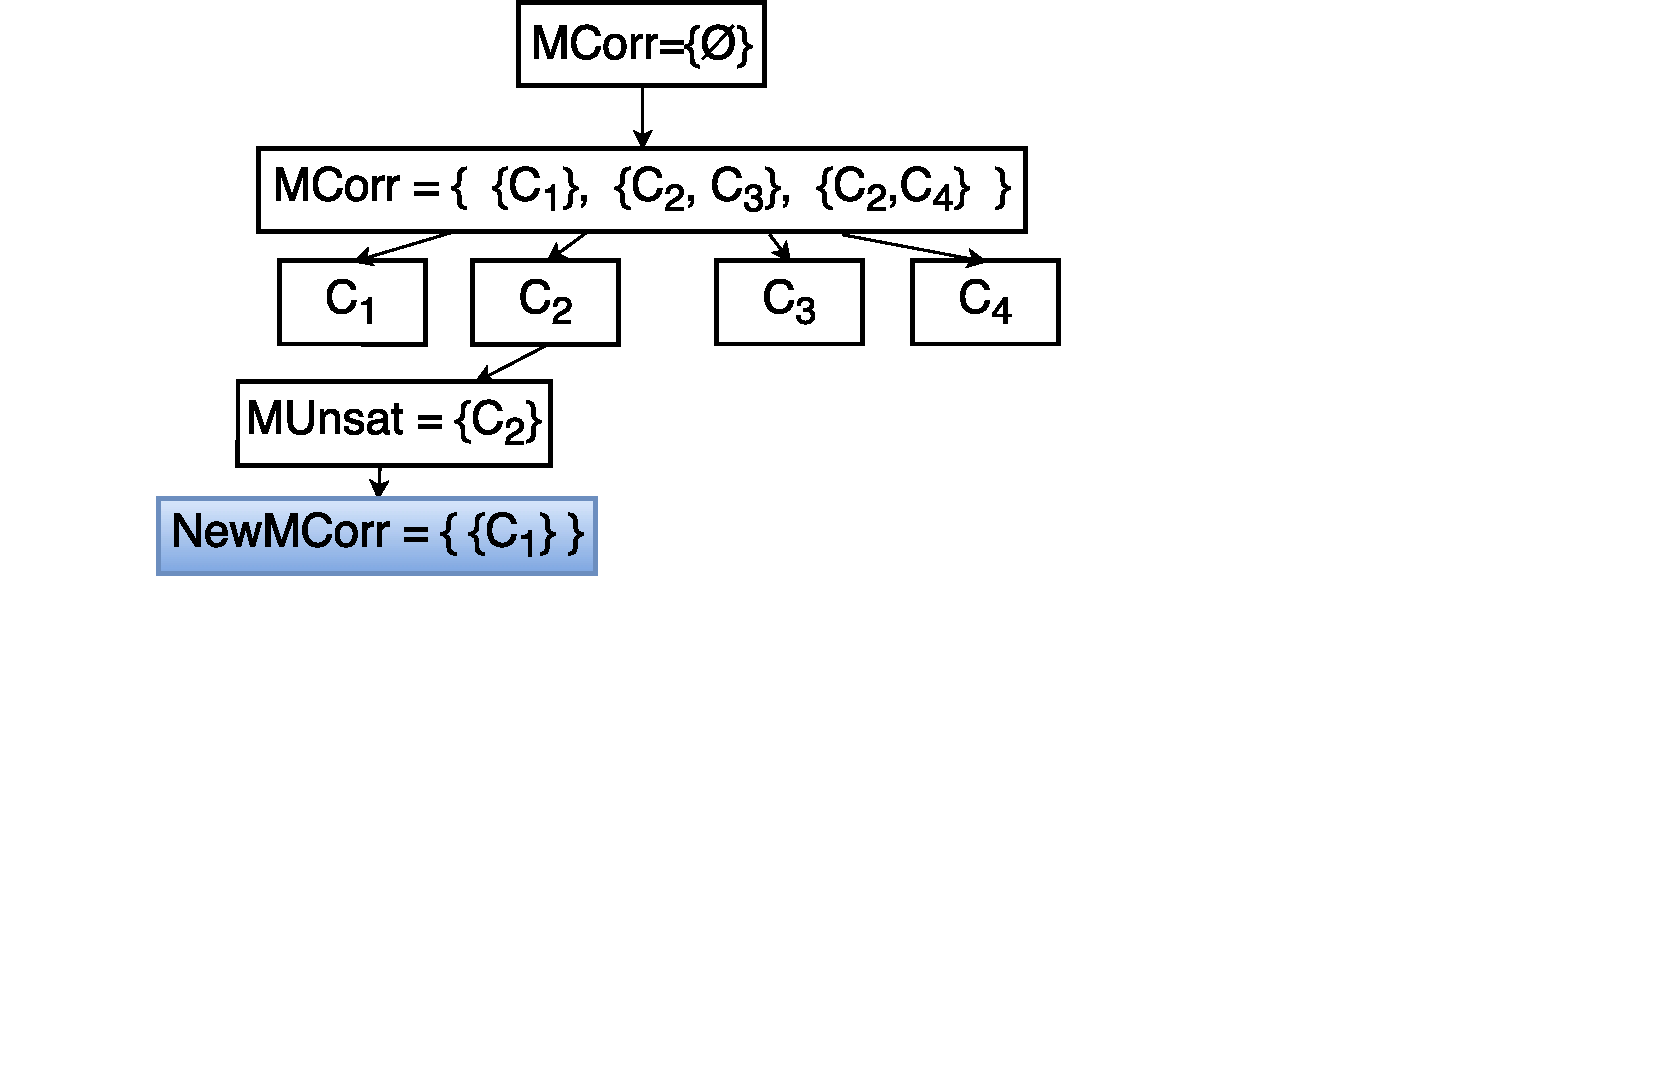
\includegraphics[scale=0.38]{HittingSetAlgo4.pdf}}
		\only<5>{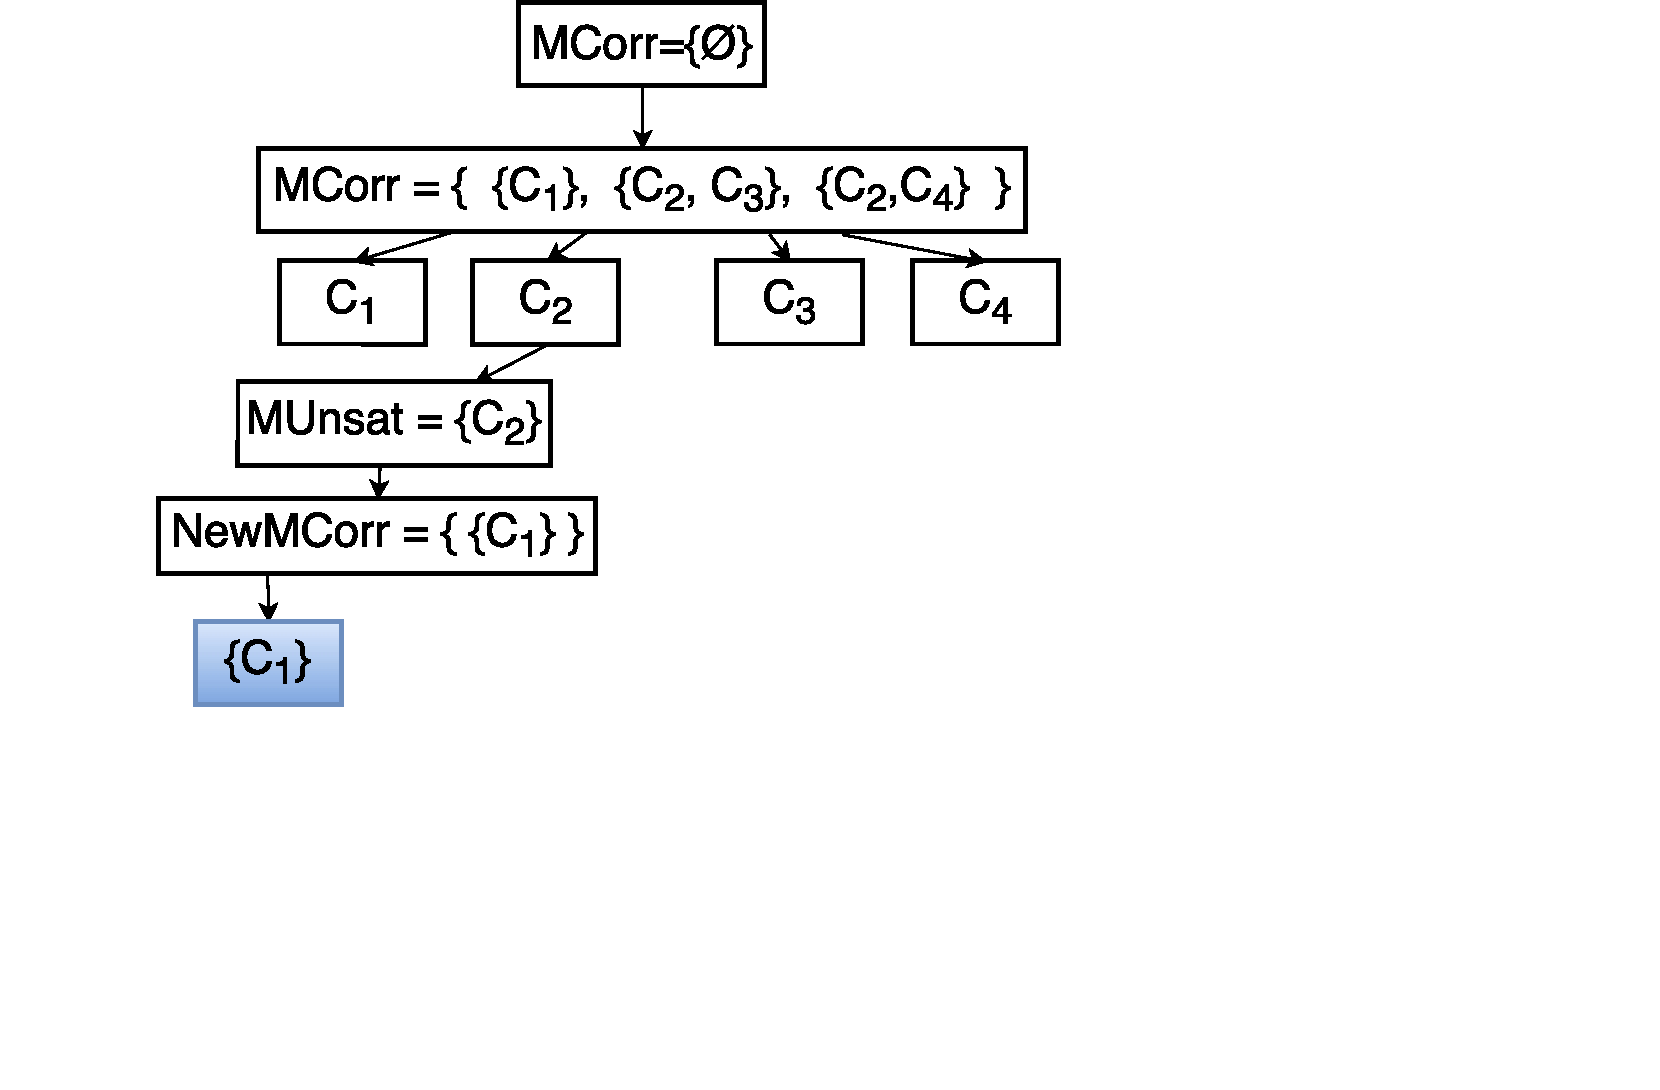
\includegraphics[scale=0.38]{HittingSetAlgo5.pdf}}
		\only<6>{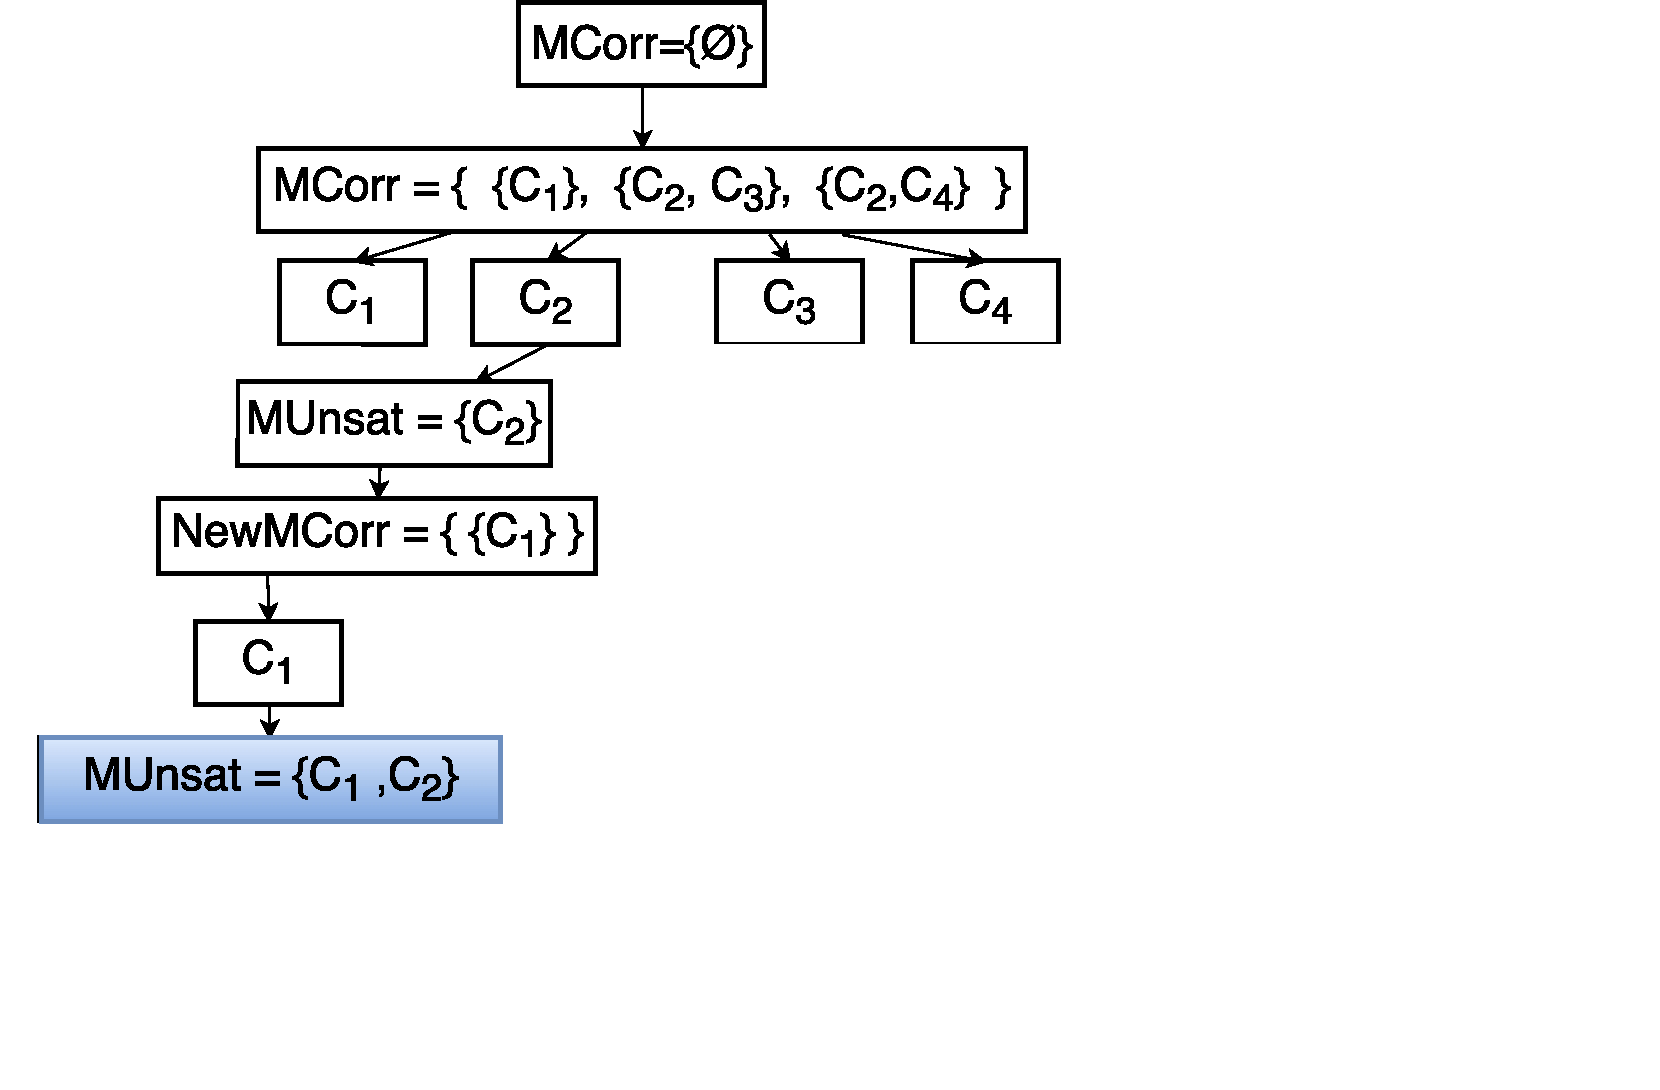
\includegraphics[scale=0.38]{HittingSetAlgo6.pdf}}
		\only<7>{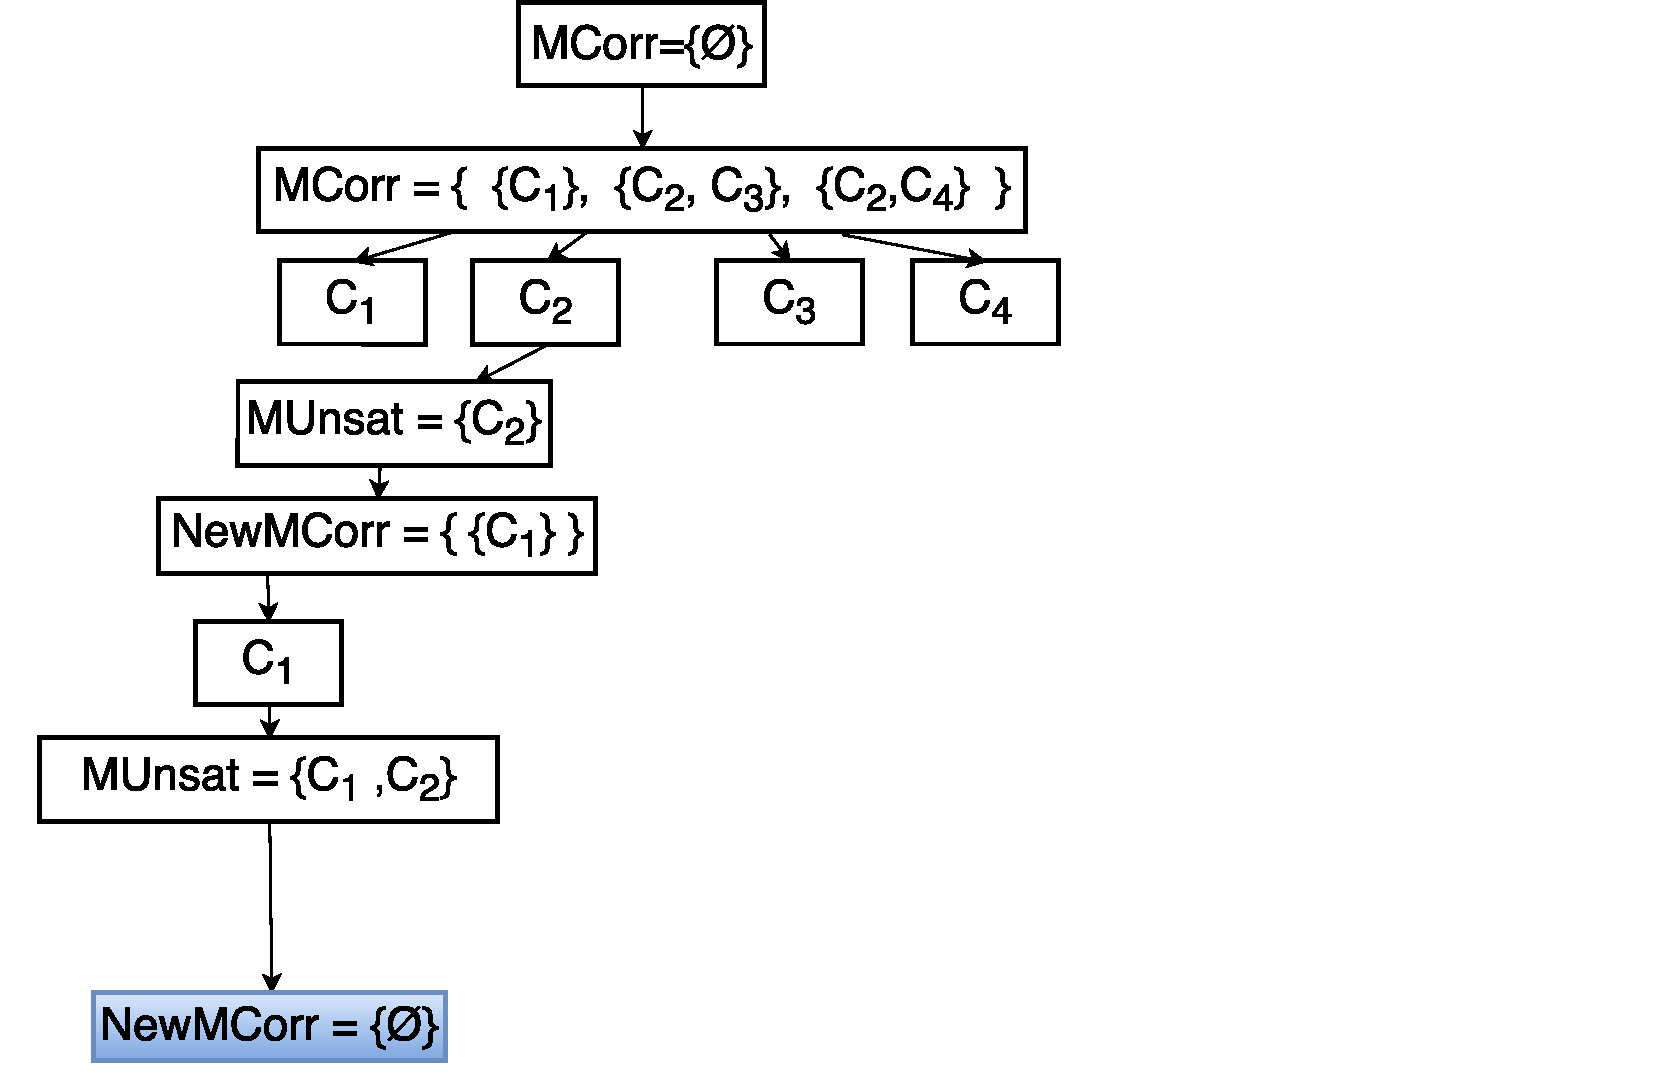
\includegraphics[scale=0.38]{HittingSetAlgo7.pdf}}
		\only<8>{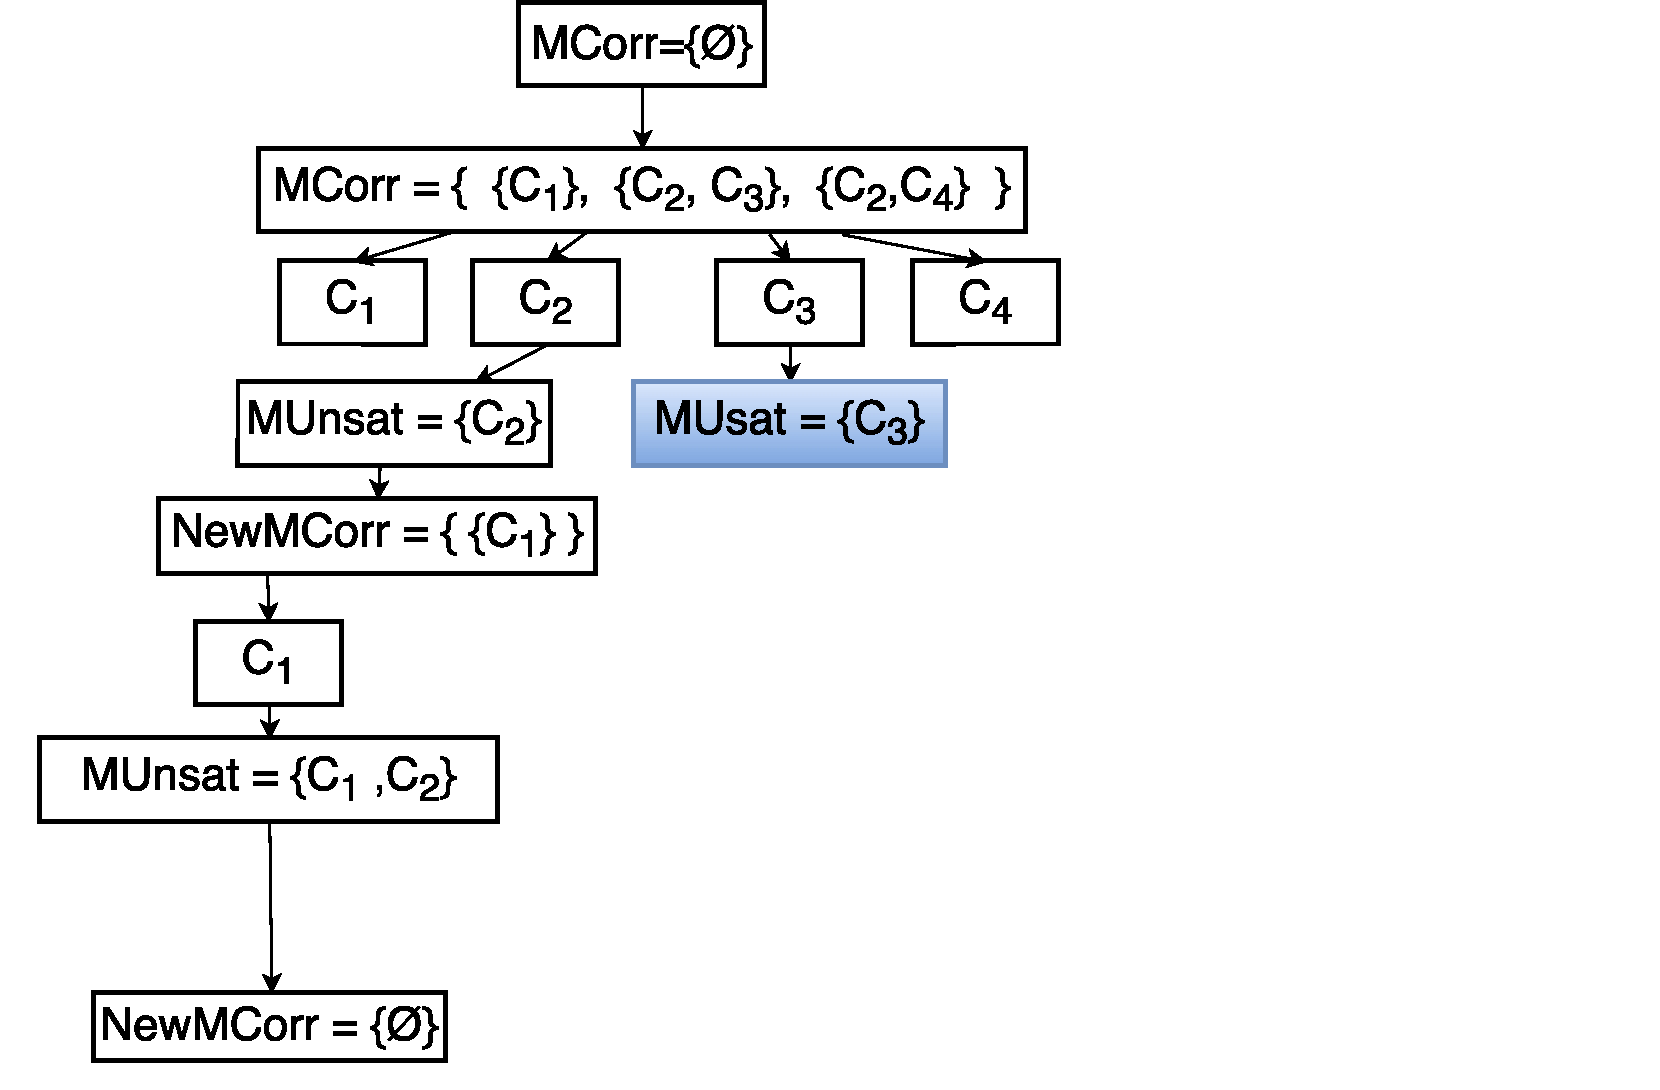
\includegraphics[scale=0.38]{HittingSetAlgo8.pdf}}
		\only<9>{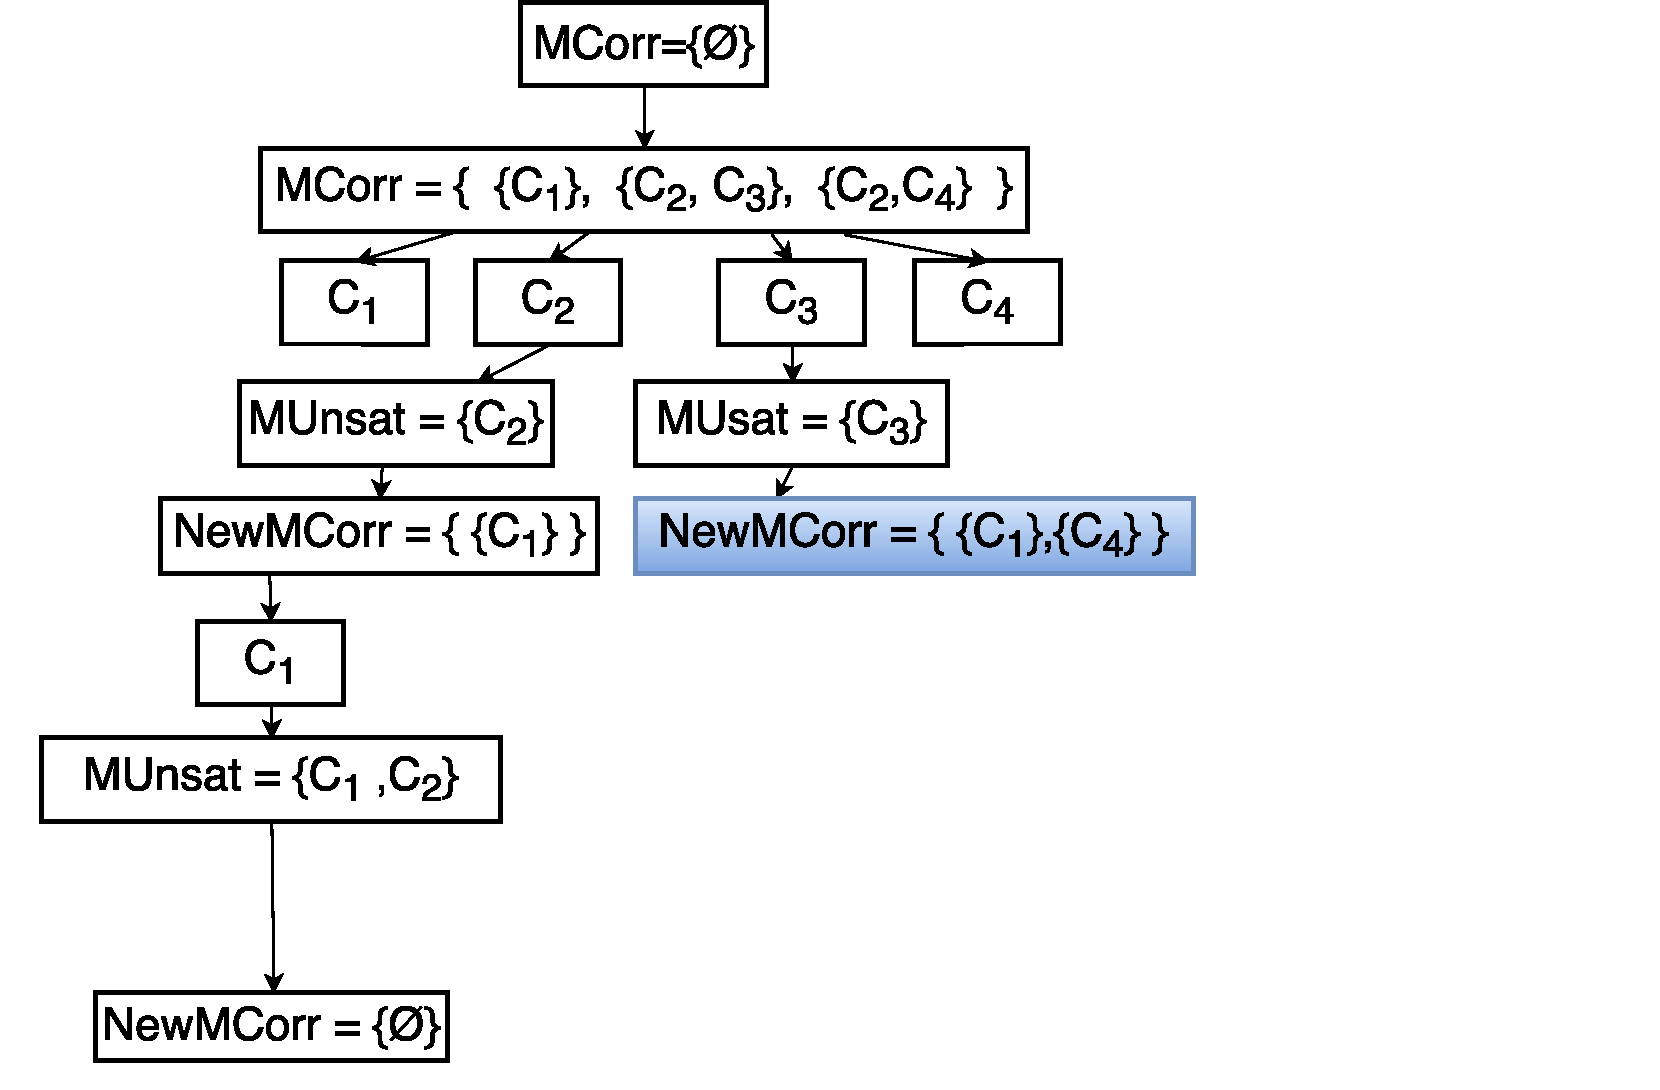
\includegraphics[scale=0.38]{HittingSetAlgo9.pdf}}
		\only<10>{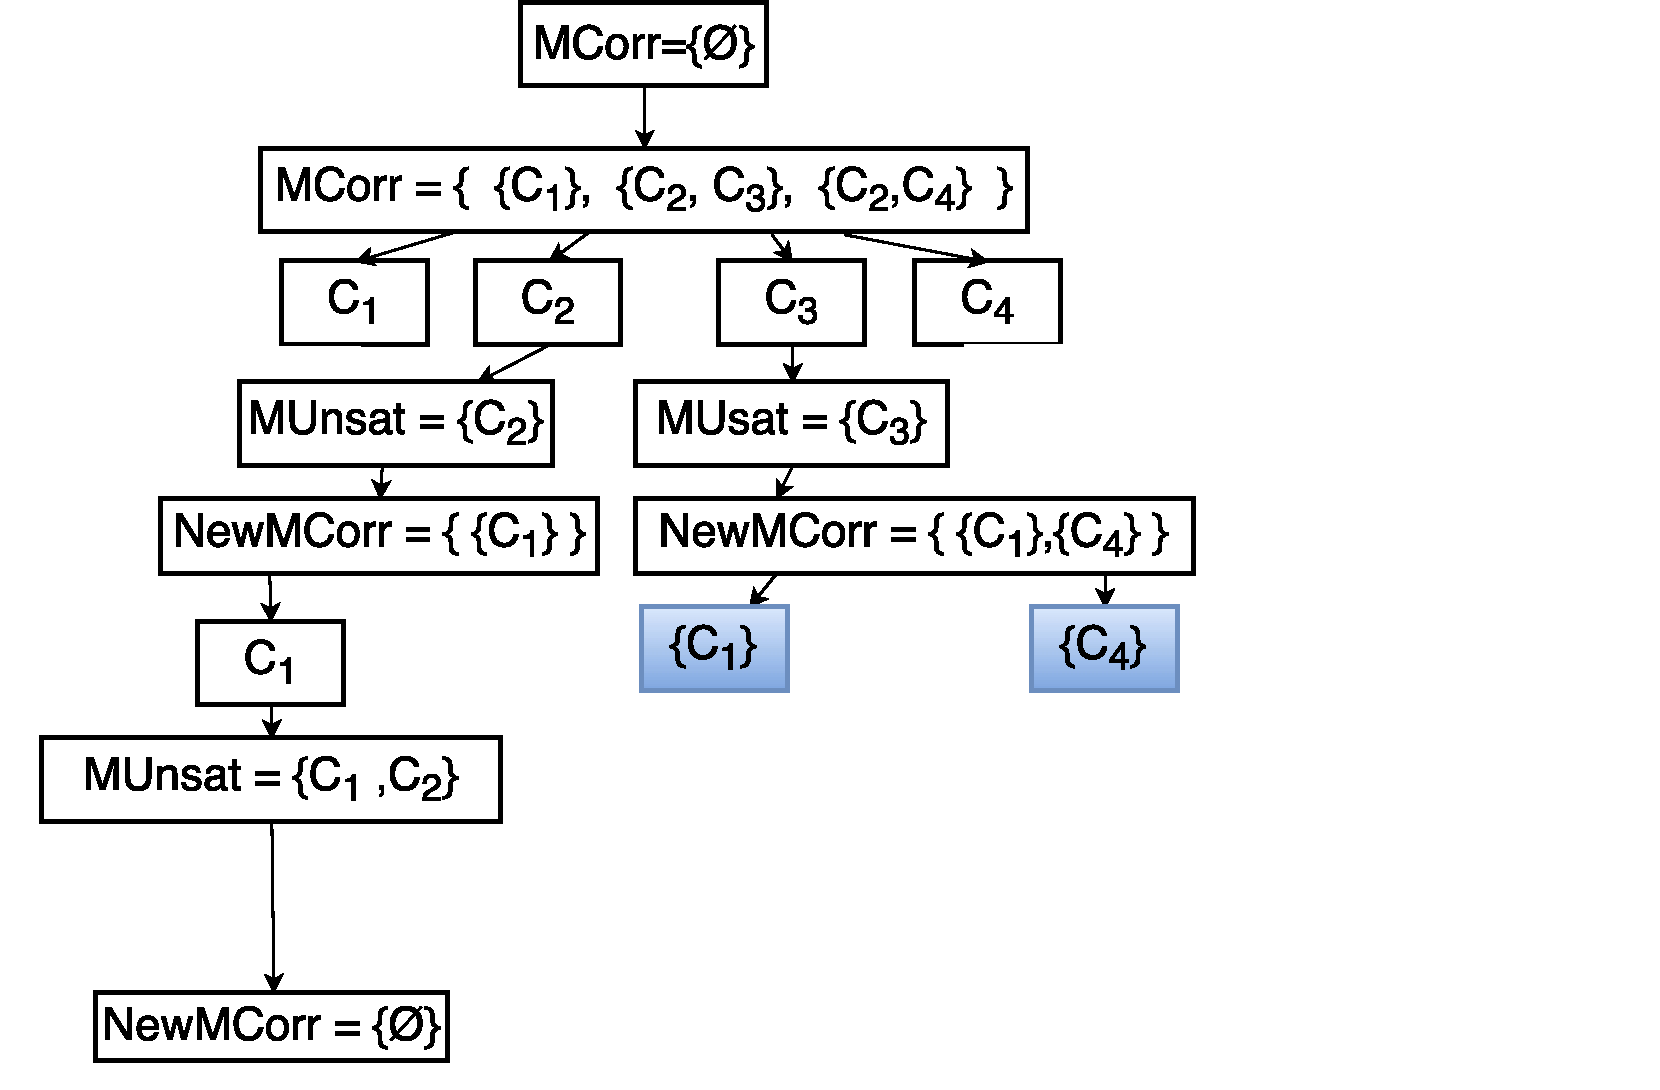
\includegraphics[scale=0.38]{HittingSetAlgo10.pdf}}
		\only<11>{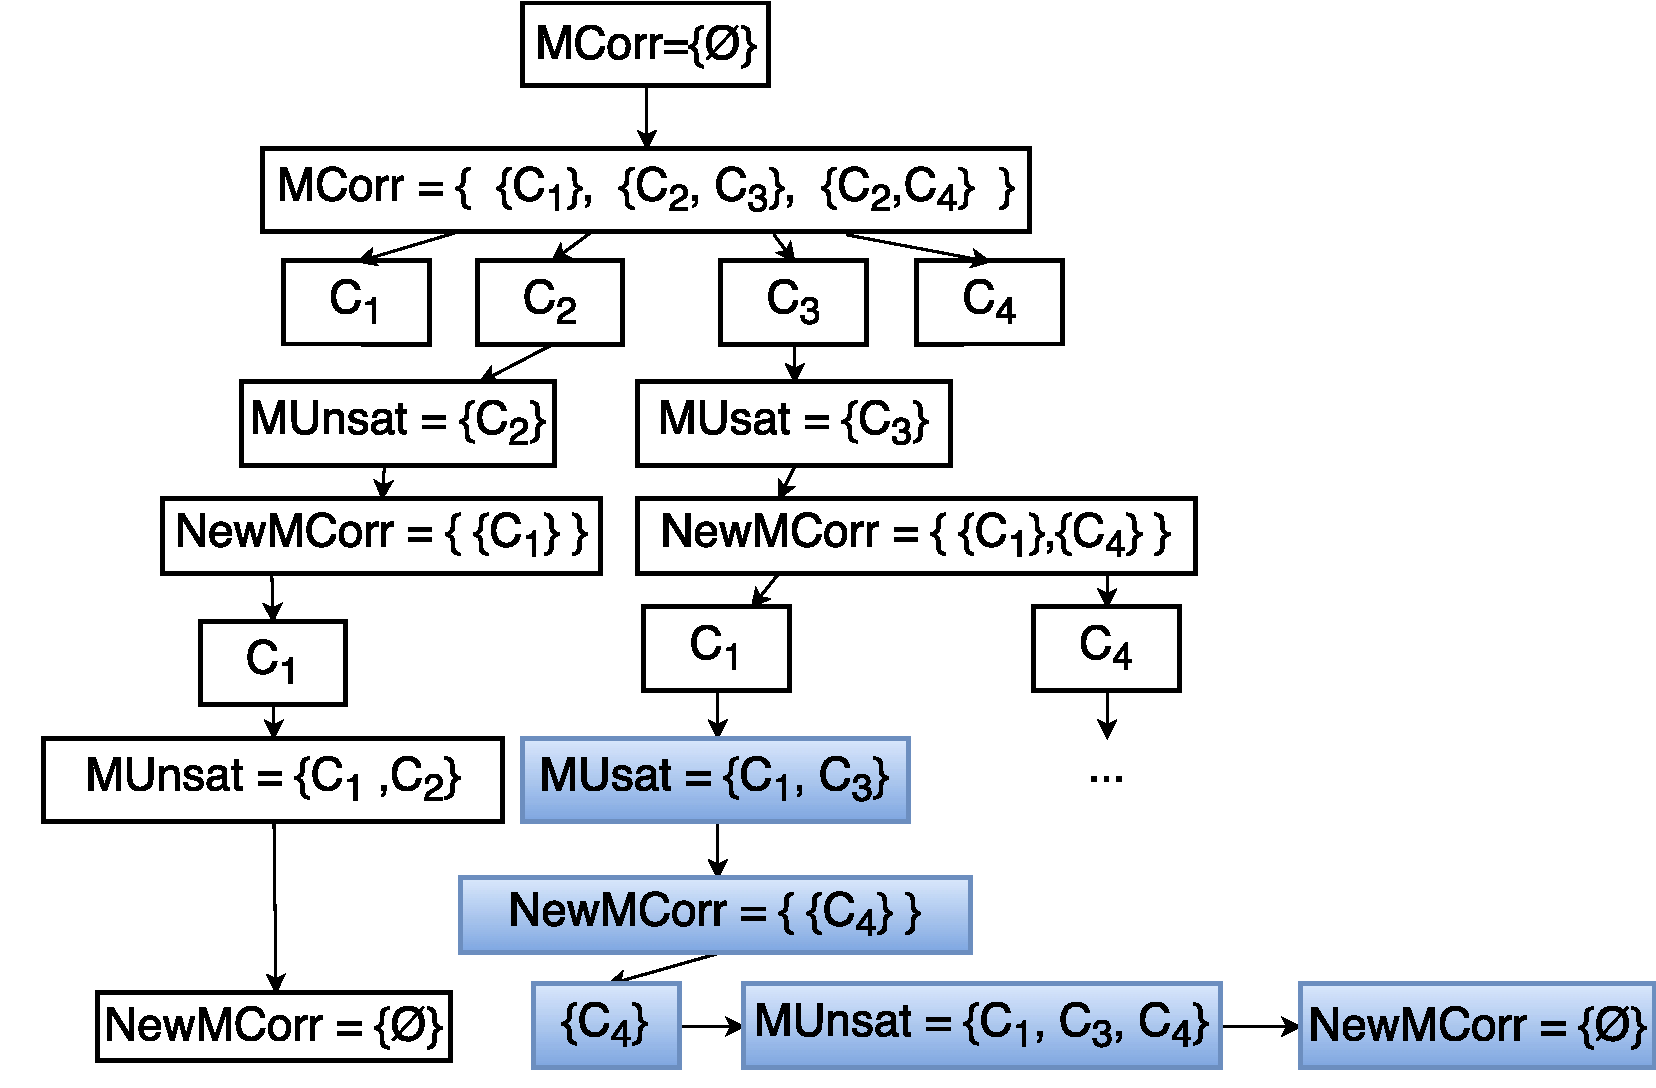
\includegraphics[scale=0.38]{HittingSetAlgo11.pdf}}
		\only<12>{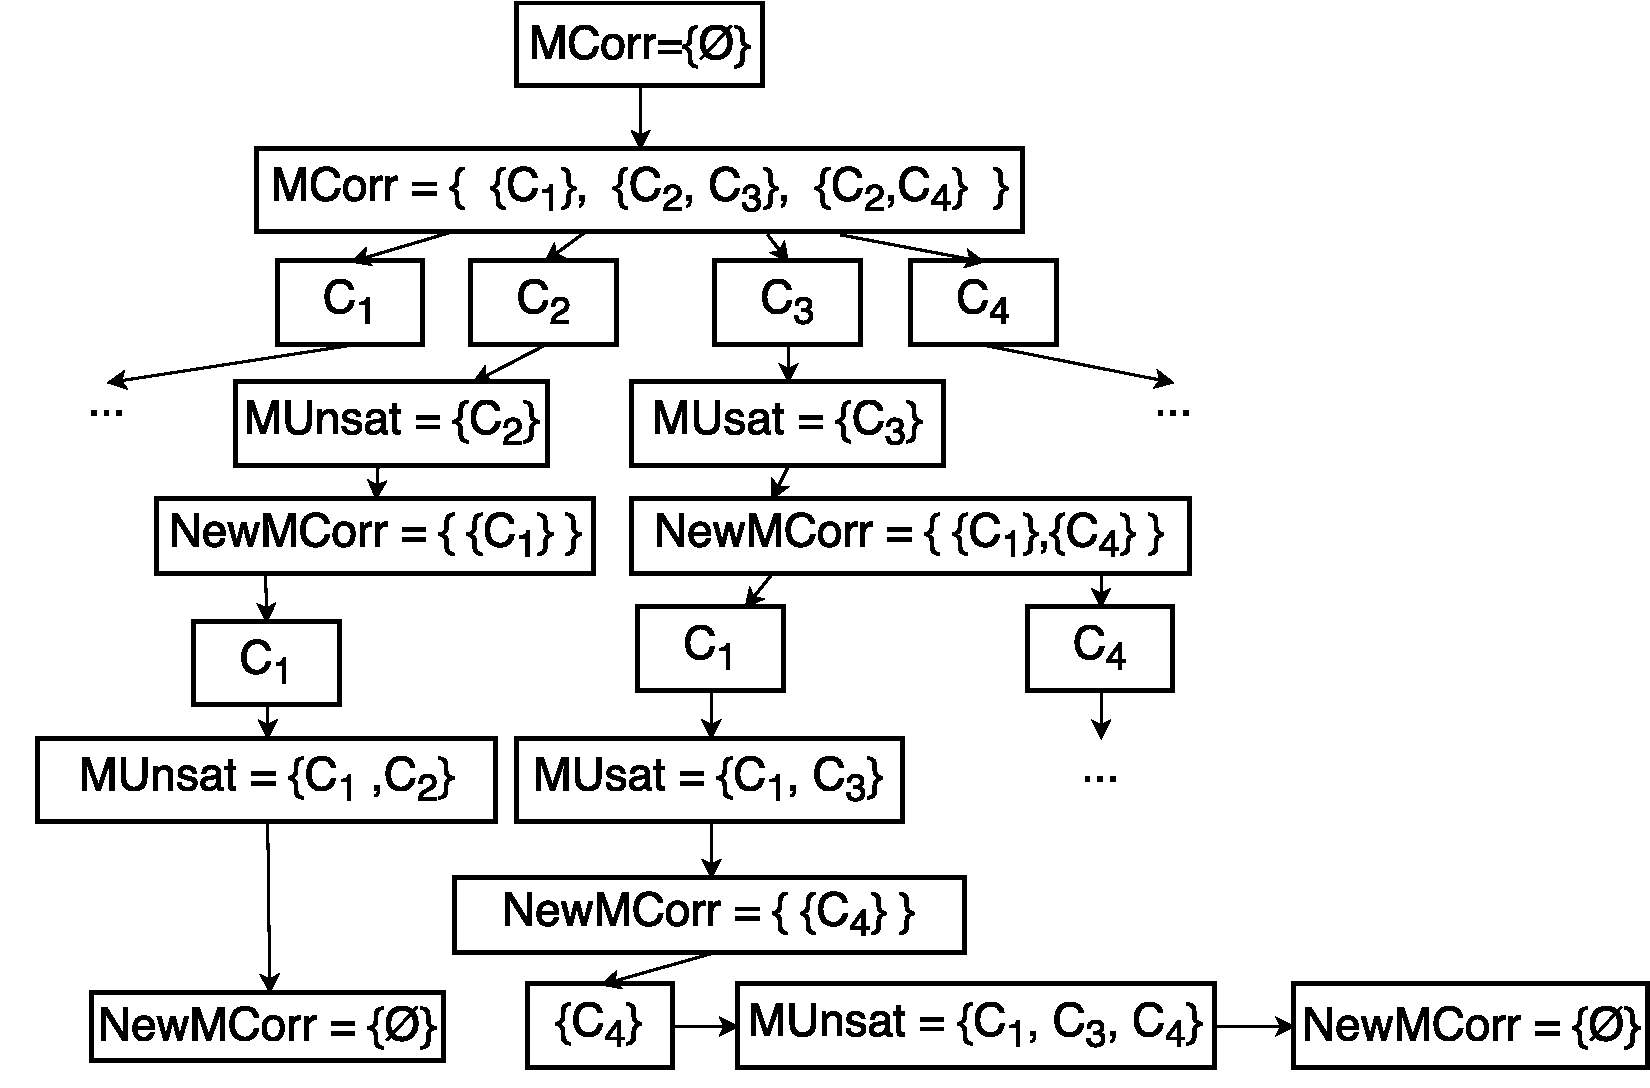
\includegraphics[scale=0.38]{HittingSetAlgo12.pdf}}
	\end{center}
\end{frame}
\begin{frame}{Reference}
\begin{thebibliography}{9}
	\bibitem{karem} 
	Mark H. Liffiton, Karem A. Sakallah,
	\textit{Algorithms for Computing Minimal Unsatisfiable Subsets of Constraints}.
	Department of Electrical Engineering and Computer Science,
	University of Michigan, Ann Arbor 48109-2121.
	\bibitem{nadel} 
	Alexander Nadel, Vadim Ryvchin, Ofer Strichman
	\textit{Ultimately Incremental SAT}.
	\url{https://ie.technion.ac.il/~ofers/publications/sat14.pdf}
\end{thebibliography}
\end{frame}
\end{document}


